% Options for packages loaded elsewhere
\PassOptionsToPackage{unicode}{hyperref}
\PassOptionsToPackage{hyphens}{url}
\PassOptionsToPackage{dvipsnames,svgnames,x11names}{xcolor}
%
\documentclass[
  singlecolumn,
  9pt]{article}

\usepackage{amsmath,amssymb}
\usepackage{iftex}
\ifPDFTeX
  \usepackage[T1]{fontenc}
  \usepackage[utf8]{inputenc}
  \usepackage{textcomp} % provide euro and other symbols
\else % if luatex or xetex
  \usepackage{unicode-math}
  \defaultfontfeatures{Scale=MatchLowercase}
  \defaultfontfeatures[\rmfamily]{Ligatures=TeX,Scale=1}
\fi
\usepackage[]{libertinus}
\ifPDFTeX\else  
    % xetex/luatex font selection
\fi
% Use upquote if available, for straight quotes in verbatim environments
\IfFileExists{upquote.sty}{\usepackage{upquote}}{}
\IfFileExists{microtype.sty}{% use microtype if available
  \usepackage[]{microtype}
  \UseMicrotypeSet[protrusion]{basicmath} % disable protrusion for tt fonts
}{}
\makeatletter
\@ifundefined{KOMAClassName}{% if non-KOMA class
  \IfFileExists{parskip.sty}{%
    \usepackage{parskip}
  }{% else
    \setlength{\parindent}{0pt}
    \setlength{\parskip}{6pt plus 2pt minus 1pt}}
}{% if KOMA class
  \KOMAoptions{parskip=half}}
\makeatother
\usepackage{xcolor}
\usepackage[top=30mm,bottom=30mm,left=20mm,heightrounded]{geometry}
\setlength{\emergencystretch}{3em} % prevent overfull lines
\setcounter{secnumdepth}{-\maxdimen} % remove section numbering
% Make \paragraph and \subparagraph free-standing
\ifx\paragraph\undefined\else
  \let\oldparagraph\paragraph
  \renewcommand{\paragraph}[1]{\oldparagraph{#1}\mbox{}}
\fi
\ifx\subparagraph\undefined\else
  \let\oldsubparagraph\subparagraph
  \renewcommand{\subparagraph}[1]{\oldsubparagraph{#1}\mbox{}}
\fi


\providecommand{\tightlist}{%
  \setlength{\itemsep}{0pt}\setlength{\parskip}{0pt}}\usepackage{longtable,booktabs,array}
\usepackage{calc} % for calculating minipage widths
% Correct order of tables after \paragraph or \subparagraph
\usepackage{etoolbox}
\makeatletter
\patchcmd\longtable{\par}{\if@noskipsec\mbox{}\fi\par}{}{}
\makeatother
% Allow footnotes in longtable head/foot
\IfFileExists{footnotehyper.sty}{\usepackage{footnotehyper}}{\usepackage{footnote}}
\makesavenoteenv{longtable}
\usepackage{graphicx}
\makeatletter
\def\maxwidth{\ifdim\Gin@nat@width>\linewidth\linewidth\else\Gin@nat@width\fi}
\def\maxheight{\ifdim\Gin@nat@height>\textheight\textheight\else\Gin@nat@height\fi}
\makeatother
% Scale images if necessary, so that they will not overflow the page
% margins by default, and it is still possible to overwrite the defaults
% using explicit options in \includegraphics[width, height, ...]{}
\setkeys{Gin}{width=\maxwidth,height=\maxheight,keepaspectratio}
% Set default figure placement to htbp
\makeatletter
\def\fps@figure{htbp}
\makeatother
% definitions for citeproc citations
\NewDocumentCommand\citeproctext{}{}
\NewDocumentCommand\citeproc{mm}{%
  \begingroup\def\citeproctext{#2}\cite{#1}\endgroup}
% avoid brackets around text for \cite:
\makeatletter
 \def\@biblabel#1{}
 \def\@cite#1#2{{#1\if@tempswa , #2\fi}}
\makeatother
\newlength{\cslhangindent}
\setlength{\cslhangindent}{1.5em}
\newlength{\csllabelwidth}
\setlength{\csllabelwidth}{3em}
\newlength{\cslentryspacing}
\setlength{\cslentryspacing}{0em}
\usepackage{enumitem}
\newlist{CSLReferences}{itemize}{1}
\setlist[CSLReferences]{label={},
  leftmargin=\cslhangindent,
  itemindent=-1\cslhangindent,
  parsep=\parskip,
  itemsep=\cslentryspacing}
\usepackage{calc}
\newcommand{\CSLBlock}[1]{#1\hfill\break}
\newcommand{\CSLLeftMargin}[1]{\parbox[t]{\csllabelwidth}{#1}}
\newcommand{\CSLRightInline}[1]{\parbox[t]{\linewidth - \csllabelwidth}{#1}\break}
\newcommand{\CSLIndent}[1]{\hspace{\cslhangindent}#1}

\usepackage{cancel}
\usepackage{xcolor}
\usepackage[noblocks]{authblk}
\renewcommand*{\Authsep}{, }
\renewcommand*{\Authand}{, }
\renewcommand*{\Authands}{, }
\renewcommand\Affilfont{\small}
\usepackage{cancel}
\usepackage{xcolor}
\makeatletter
\makeatother
\makeatletter
\makeatother
\makeatletter
\@ifpackageloaded{caption}{}{\usepackage{caption}}
\AtBeginDocument{%
\ifdefined\contentsname
  \renewcommand*\contentsname{Table of contents}
\else
  \newcommand\contentsname{Table of contents}
\fi
\ifdefined\listfigurename
  \renewcommand*\listfigurename{List of Figures}
\else
  \newcommand\listfigurename{List of Figures}
\fi
\ifdefined\listtablename
  \renewcommand*\listtablename{List of Tables}
\else
  \newcommand\listtablename{List of Tables}
\fi
\ifdefined\figurename
  \renewcommand*\figurename{Figure}
\else
  \newcommand\figurename{Figure}
\fi
\ifdefined\tablename
  \renewcommand*\tablename{Table}
\else
  \newcommand\tablename{Table}
\fi
}
\@ifpackageloaded{float}{}{\usepackage{float}}
\floatstyle{ruled}
\@ifundefined{c@chapter}{\newfloat{codelisting}{h}{lop}}{\newfloat{codelisting}{h}{lop}[chapter]}
\floatname{codelisting}{Listing}
\newcommand*\listoflistings{\listof{codelisting}{List of Listings}}
\makeatother
\makeatletter
\@ifpackageloaded{caption}{}{\usepackage{caption}}
\@ifpackageloaded{subcaption}{}{\usepackage{subcaption}}
\makeatother
\makeatletter
\makeatother
\ifLuaTeX
  \usepackage{selnolig}  % disable illegal ligatures
\fi
\IfFileExists{bookmark.sty}{\usepackage{bookmark}}{\usepackage{hyperref}}
\IfFileExists{xurl.sty}{\usepackage{xurl}}{} % add URL line breaks if available
\urlstyle{same} % disable monospaced font for URLs
\hypersetup{
  pdftitle={Causal Diagrams for the Evolutionary Human Sciences: A Practical Guide},
  pdfauthor={Joseph A. Bulbulia},
  pdfkeywords={Directed Acyclic Graph, Causal
Inference, Confounding, Feedback, Interaction, Mediation, Moderation, Panel},
  colorlinks=true,
  linkcolor={blue},
  filecolor={Maroon},
  citecolor={Blue},
  urlcolor={Blue},
  pdfcreator={LaTeX via pandoc}}

\title{Causal Diagrams for the Evolutionary Human Sciences: A Practical
Guide}


  \author{Joseph A. Bulbulia}
            \affil{%
                  Victoria University of Wellington, New Zealand, School
                  of Psychology, Centre for Applied Cross-Cultural
                  Research
              }
      
\date{2023-11-30}
\begin{document}
\maketitle
\begin{abstract}
Causation inherently unfolds in time. However, quantifying a causal
effect relies on contrasting counterfactual states of the world that
never occur. As such, causal data science relies on explicit assumptions
and careful, multi-stepped workflows. Within this framework, causal
diagrams have been developed as powerful tools for evaluating structural
assumptions necessary for obtaining consistent causal effect estimates
from data. However, outside this framework, causal diagrams may be
easily misinterpreted and misused. This guide offers practical advice
for creating safe, effective causal diagrams. I begin by reviewing the
causal data science framework, clarifying how causal diagrams function
within it. Next, I develop a series of examples that illustrate the
benefits of chronological order in the spatial organisation of one's
graph, both for data analysis and collection. I conclude using
chronologically ordered causal diagrams to elucidate the widely
misunderstood concepts of interaction (moderation), mediation, and
dynamic longitudinal feedback.
\end{abstract}
\subsection{Introduction}\label{introduction}

Correlation does not imply causation. This adage is widely known.
Nevertheless, many human scientists report manifest correlations and use
hedging language that implies causation. I have been guilty. However,
such reporting typically lacks justification. Making matters worse,
widely adopted analytic strategies for confounding control, such as
indiscriminate co-variate adjustment, are known to enhance bias
(\citeproc{ref-mcelreath2020}{McElreath 2020}). Across many human
sciences, including the evolutionary human sciences, persistent
confusion in the analysis and reporting of correlations continue to
impede scientific progress -- suggesting a causality crisis.

We have reasons for hope. First, the open science movement has
demonstrated that attention to the problems of replication, analysis,
and reporting can bring considerable improvements to the reliability of
experimental research within a short period. Although much remains to be
done, and it is easy to focus on headroom for improvement, basic
corrective practices for open science have become normative. Moreover,
the system of rewards that supports research has changed, for example,
by the peer review of research designs rather than of results. Again,
there is much scope for improvement, but this should not detract from
the progress achieved. Second, several decades of active development in
the causal data sciences across the health sciences, computer sciences,
economics, and several social sciences have yielded both considerable
conceptual clarifications and rigorous analytic toolkits for inference
(\citeproc{ref-hernan2023}{Hernan and Robins 2023};
\citeproc{ref-neyman1923}{Neyman 1923}; \citeproc{ref-pearl2009a}{Pearl
2009b}; \citeproc{ref-pearl1995}{Pearl and Robins 1995a};
\citeproc{ref-robins1986}{Robins 1986}; \citeproc{ref-rubin1976}{Rubin
1976}; \citeproc{ref-vanderweele2015}{VanderWeele 2015}). Although
causal data science is still evolving (\citeproc{ref-duxedaz2021}{Díaz
\emph{et al.} 2021}; \citeproc{ref-hoffman2023}{Hoffman \emph{et al.}
2023}; \citeproc{ref-vansteelandt2022}{Vansteelandt and Dukes 2022}), a
substantial foundation exists. Importantly, this foundation is written
in a system of mathematical proofs that bring confidence. Indeed, there
are encouraging examples of convergent evolution across pockets of
development. Most debates within causal data science are peripheral to
its core conceptual framework. We can, with reasonable justification,
speak of causal data science in the singular. Although exciting
developments remain ahead, essential concepts, theories, and tools have
already been worked out. We should be optimistic that rapid uptake of
these tools is feasible. The articles in this special issue of
\emph{Evolutionary Human Sciences} testify to this hope.

Within the framework of causal data science, causal diagrams, also known
as `directed acyclic graphs' or `DAGs,' have been developed as powerful
inferential tools. Their applications rest on a robust system of formal
mathematical proofs that should instil confidence. Nevertheless, they do
not require mathematical training and are broadly accessible. This
accessibility is a great advantage.

However, the accessibility that empowers causal diagrams to improve our
causal inferences also invites risks. The tool acquires its significance
when integrated within the broader theoretical frameworks of causal data
science. This framework distinguishes itself from traditional data
science by attempting to estimate pre-specified contrasts, or
`estimands', among counterfactual states of the world. However, we
assume these counterfactual states to be real they never occur. Instead,
the required counterfactual scenarios are simulated from data under
explicit assumptions that must be justified
(\citeproc{ref-edwards2015}{Edwards \emph{et al.} 2015};
\citeproc{ref-robins1986}{Robins 1986};
\citeproc{ref-vansteelandt2012}{Vansteelandt \emph{et al.} 2012}). These
\emph{structural assumptions} differ from the statistical assumptions
familiar to traditionally trained data scientists and computer
scientists. Because causal data scientists must eventually use
statistical models, careful statistical validations must also enter the
workflow. We cannot assume that traditionally trained human scientists,
even those with excellent statistical trading, have familiarity with the
demands of counterfactual inference, in which the data we observe
provide inherently partial insights into the targeted counterfactual
contrasts and their uncertainties (\citeproc{ref-bulbulia2023}{Bulbulia
2023}; \citeproc{ref-ogburn2021}{Ogburn and Shpitser 2021}). Using
causal diagrams without understanding their role within the framework of
theory and assumptions that underpin causal data science risks
inadvertently worsen the causality crisis by fostering misguided
confidence where none is due.

Here, I offer readers of \emph{Evolutionary Human Science} practical
guidance for creating causal diagrams that work as we hope while
mitigating risks of overreaching.

\textbf{Part 1} introduces certain core concepts and theories in causal
data science, emphasising fundamental assumptions and the demands they
impose on inferential workflows. Although this overview is brief, it
provides an orientation to the broader context in which causal diagrams
possess their utility, outside of which the application of causal
diagrams offers no guarantees.

\textbf{Part 2} introduces \emph{chronologically ordered causal
diagrams} and considers elementary use cases. Here, I illustrate how
maintaining `chronological hygiene' in the spatial layout of a causal
diagram is helpful not only for the tasks of developing sound
data-analytic strategies but also for research planning and data
collection. Although chronological ordering is not strictly essential
and indeed is not widely practised, the examples I consider demonstrate
its advantages in common scenarios.

\textbf{Part 3} uses chronologically ordered causal diagrams, applied
within the broader framework of causal data science, to demystify
misunderstood concepts of interaction (moderation), mediation, and
longitudinal data analysis. Again, the frameworks of causal data science
are indispensable for clarifying the quantities researchers hope to
understand when applying statistical models to questions of interaction,
mediation, and dynamic longitudinal feedback. We again discover that
maintaining good chronological hygiene in one's causal diagram benefits
data analysis and collection. We also discover that in many commonplace
settings, seemingly accessible questions, such as `How much of total
effect is mediated?' cannot be directly evaluated by the data, even at
the limit of perfect data collection. Unfortunately, questions of
interaction, mediation, and longitudinal feedback remain poorly served
by analytic traditions in which many human scientists and statisticians
were trained, such as the structural equation modelling tradition (SEM).
These traditions continue to dominate, yet we can do better and should.

There are numerous excellent resources available for learning causal
diagrams, which I recommend to readers
(\citeproc{ref-barrett2021}{Barrett 2021};
\citeproc{ref-cinelli2022}{Cinelli \emph{et al.} 2022};
\citeproc{ref-greenland1999}{Greenland \emph{et al.} 1999a};
\citeproc{ref-hernan2023}{Hernan and Robins 2023};
\citeproc{ref-mcelreath2020}{McElreath 2020};
\citeproc{ref-pearl2009}{Pearl 2009a}; \citeproc{ref-rohrer2018}{Rohrer
2018}; \citeproc{ref-suzuki2020}{Suzuki \emph{et al.}
2020a}).\footnote{An excellent resource is Miguel Hernán's free online
  course, here:
  \url{https://pll.harvard.edu/course/causal-diagrams-draw-your-assumptions-your-conclusions}.}
I hope to contribute to these resources, first by providing additional
conceptual orientation to the frameworks and workflows of causal data
science, outside of which the application of causal diagrams is risky;
second, by underscoring the benefits of chronological hygiene in one's
causal diagrams for common problems; and third by applying this
orientation to concepts of interaction, mediation, and longitudinal
feedback, about which there remains considerable confusions.

\subsection{Part 1. Overview of Causal Data
Science}\label{part-1.-overview-of-causal-data-science}

In causal data science, the critical first step in answering a causal
question is to ask it (\citeproc{ref-hernuxe1n2016}{Hernán \emph{et al.}
2016}). Causal diagrams come later when we consider which forms of data
might enable us to address our pre-specified causal questions. This
section introduces the key concepts and broader workflows within which
causal diagrams find their purposes and utilities. It begins by
considering what is at stake when we ask a causal question.

\subsubsection{The Fundamental Problem of Causal
Inference}\label{the-fundamental-problem-of-causal-inference}

To ask a causal question, we must consider the concept of causality
itself. Consider an intervention, \(A\), and its effect, \(Y\). We say
that \(A\) causes \(Y\) if altering \(A\) would lead to a change in
\(Y\) (\citeproc{ref-hume1902}{Hume 1902};
\citeproc{ref-lewis1973}{Lewis 1973}). If altering \(A\) would not
change \(Y\), we say that \(A\) has no causal effect on \(Y\).

In causal data science, we aim to quantitatively contrast in a
well-defined outcome \(Y\) when subjected to different levels of a
well-defined intervention \(A\). Commonly, we refer to these
interventions as `exposures' or `treatments;' we refer to the possible
effects of interventions as `potential outcomes.'

Let us assume that \(A\) exists in two states: \(A \in \{0,1\}\). If
\(A\) is set to \(0\) we denote the potential outcome as \(Y(0)\). If
\(A\) is set to 1, we denote the potential outcome as \(Y(1)\). We call
\(Y(1), Y(0)\) `potential outcomes' because, until realised, the
outcomes are counterfactual.

Next suppose we have stated a well-defined exposure and outcome. Each
unit, \(i \dots, n\), can either experience \(Y_i|A_i = 1\) or
\(Y_i|A_i = 0\). For any realised intervention we cannot observe the
unrealised intervention. As a result, we cannot directly calculate a
contrast between \(Y_i(1)\) and \(Y_i(0)\) from observable data.:

-If \(A_i = 1\), the outcome under treatment is observed
(\(Y_i(1)|A_i=1\)), but the outcome under no treatment remains
unobserved (\(Y_i(0)|A_i=1\)). This can be expressed as:

\[
Y_i|A_i = 1 \implies Y_i(1)|A_i=0~ \text{is counterfactual}
\]

Conversely, if \(A = 0\), the outcome under no treatment is observed:
\(Y_i(0)|A=0\), but the outcome under treatment is unobserved:
\(Y_i(1)|A=0\). This constraint can be expressed as:

\[
Y_i|A_i = 0 \implies Y(0)|A=1~ \text{is counterfactual} 
\]

Where \(\delta_i\) is the quantity of interest,

\[
\delta_i = Y_i(1) - Y_i(0)
\]

We discover \(\delta_i\) is unobservable: each unit can receive only one
exposure at one time.

This framework highlights the fundamental challenge of causal inference,
where one of the potential outcomes is always missing. The fact that
individual causal effects are not identified from observations is
``\emph{the fundamental problem of causal inference}''
(\citeproc{ref-holland1986}{Holland 1986};
\citeproc{ref-rubin1976}{Rubin 1976}).

We are familiar with the inaccessibility of counterfactuals. It may be
tempting to ask, `What if Isaac Newton had not observed the falling
apple?' `What if Leonardo da Vinci had never pursued art?' or `What if
Archduke Ferdinand had not been assassinated?' We have many examples
from literature. Frost contemplates, `Two roads diverged in a yellow
wood, and sorry I could not travel both, and be one traveller, long I
stood\ldots{}'\footnote{see: Robert Frost, ``The Road Not Taken'':
  https://www.poetryfoundation.org/poems/44272/the-road-not-taken} We
have examples from personal experience, `What if I had had not
interviewed for that job?' `What if I had stayed in that relationship?'
We may speculate, with reasons, but we cannot directly observe the
answers. The physics of middle-sized dry goods prevents the joint
realisations of the facts required for comparisons.

A distinctive feature of causal data science is the assumption that,
although never jointly realised, the potential outcomes \(Y(1),Y(0)\)
must nevertheless be assumed to be real, and to exist independently of
data collection.\footnote{As Hernán and Robins point out: ``Sometimes we
  abbreviate the expression individual \(i\) has outcome \(Y^a = 1\) by
  writing \(Y^a_i = 1\). Technically, when \(i\) refers to a specific
  individual, such as Zeus, \(Y^a_i\) is not a random variable because
  we are assuming that individual counterfactual outcomes are
  deterministic\ldots{} Causal effect for individual
  \(i: Y^{a=1}\neq Y^{a=0}\)'' (\citeproc{ref-hernan2023}{Hernan and
  Robins 2023 p. 6})} As such, causal data science faces a unique type
of missing data problem in which the `full data' needed to compute any
causal contrast are missing at least half of their values
(\citeproc{ref-edwards2015}{Edwards \emph{et al.} 2015};
\citeproc{ref-ogburn2021}{Ogburn and Shpitser 2021};
\citeproc{ref-westreich2015}{Westreich \emph{et al.} 2015}). This
challenge is distinct from typical missing data scenarios where data
could have been recorded but were not. The missing information crucial
for computing causal contrasts is intrinsically linked to the
irreversible nature of time.

\subsubsection{Obtaining Average Causal Effects From
Observations}\label{obtaining-average-causal-effects-from-observations}

In typical scenarios, computing individual causal effects is not
feasible. However, it is possible to calculate average causal effects
under certain assumptions. That is, we may obtain \emph{average}
treatment effects by contrasting groups that have received different
levels of treatment. On a difference scale, the average treatment effect
(\(\Delta_{ATE}\))) may be expressed,

\[
\Delta_{ATE}  = \mathbb{E}[Y(1)] - \mathbb{E}[Y(0)]
\]

Rearranging, \(\mathbb{E[(Y(1)-Y(0))|A]}\) denotes the expected average
difference in the responses of all individuals within an exposure group,
and \(Y(1)\) and \(Y(0)\) represent the potential outcomes under
interventions \(A = 1\) and \(A = 0\), respectively. (We drop the
subscripts to simplify notation).

Given that individual causal effects are not observable -- they are
missing -- how might we compute these averages? We do so with
assumptions. To understand how it is helpful to consider how randomised
experiments obtain contrasts of averages between treatment assignment
groups.

First, let us state the problem in terms of the `full data' we would
need to base these contrasts on observations. Where ATE denotes the
``Average Treatment Effect'':

\[
\Delta_{ATE} = \left(\underbrace{\underbrace{\mathbb{E}[Y(1)|A = 1]}_{\text{observed for } A = 1} + \underbrace{\mathbb{E}[Y(1)|A = 0]}_{\text{unobserved for } A = 0}}_{\text{effect among treated}}\right) - \left(\underbrace{\underbrace{\mathbb{E}[Y(0)|A = 0]}_{\text{observed for } A = 0} + \underbrace{\mathbb{E}[Y(0)|A = 1]}_{\text{unobserved for } A = 1}}_{\text{effect among untreated}}\right)
\]

In each treatment condition assignment, the potential outcome for each
unit that did not receive the opposite level of treatment they, in fact
received is missing. However, when researchers randomise units into
treatment conditions, the distributions of the confounders of the
potential outcomes cancel each other out. When treatments are randomly
assigned, and randomisation is effective, the outcomes under different
treatment conditions should be identical in expectation.

\[
 \mathbb{E}[Y(0) | A = 1] = \mathbb{E}[Y(0) | A = 0] 
\]

\[
\mathbb{E}[Y(1) | A = 1] = \mathbb{E}[Y(1) | A = 0] 
\]

And thus,

\[
  \widehat{\Delta_{ATE}} = \mathbb{E}[Y | A = 1] - \mathbb{E}[Y | A = 0]
\]

Here, \(\widehat{\Delta_{ATE}}\) provides an unbiased estimate of
average treatment effect on the difference scale.

Although randomisation can fail, it provides a means to identify
group-level causal effects using a Sherlock-Holmes-like process of
inference by elimination. The distribution of potential outcomes must
the same across treatment groups because randomisation in an ideally
conducted experiment exhausts every other explanation except the
treatment. For this reason, we should prefer experiments for addressing
causal questions that experiments can address.

Alas, randomised experiments cannot address many of the most important
scientific questions. This limitation is acutely felt when evolutionary
human scientists confront `what if?' scenarios rooted in the
unidirectional nature of human history. However, understanding how
randomisation obtains missing counterfactual outcomes clarifies the
tasks of causal inference in non-experimental settings
(\citeproc{ref-hernuxe1n2008a}{Hernán \emph{et al.} 2008};
\citeproc{ref-hernuxe1n2022}{Hernán \emph{et al.} 2022a};
\citeproc{ref-hernuxe1n2006}{Hernán and Robins 2006}). We must obtain
balance across observed variables that might account for treatment-level
differences (\citeproc{ref-greifer2023}{Greifer \emph{et al.} 2023}).
This task of obtaining balance presents a significant challenge
(\citeproc{ref-stuart2015}{Stuart \emph{et al.} 2015}). Observations
typically cannot in themselves verify no-unmeasured confounding.

Moreover, we must satisfy ourselves with additional assumptions, which,
although nearly automatic in randomised experimental settings, impose
substantial restrictions on causal effect estimation where the exposure
is not randomised. We next discuss a subset of these assumptions and
group them into two categories: (1) Fundamental identification
assumptions; (2) Practical assumptions. We will locate the primary
functions of causal diagrams within a workflow that must explicitly
clarify a pathway for satisfying them.

\subsubsection{Fundamental Identification
Assumptions}\label{fundamental-identification-assumptions}

There are three fundamental identification assumptions that must be
satisfied to consistently estimate causal effects with data. \#\#\#\#
Assumption 1: Causal Consistency

The causal consistency assumption posits that for any given level of
exposure, \(A_i=a\), the observed outcome, \(Y_i|A_i=a\), is
interchangeable with the counterfactual outcome: \(Y(a)|A = a\). To
illustrate, we use the subscript \(i\) to represent individual
\(i, 1 \dots n\). We define the observed outcome when treatment is
\(A_i = a\) as \(Y_i^{observed}|A_i = a\). When the causal consistency
assumption is satisfied, we say the observed outcome for each
\(i, 1 \dots n\) corresponds to one of the counterfactual outcomes
necessary for calculating a causal contrast:

\[
Y_i^{observed}|A_i = 
\begin{cases} 
Y_i(a^*) & \text{if } A_i = a^* \\
Y_i(a) & \text{if } A_i = a
\end{cases}
\]

The consistency assumption implies that the observed outcome at a
specific exposure level mirrors the counterfactual outcome for that
individual. Although it seems straightforward to equate an individual's
observed outcome with their counterfactual outcome, treatment conditions
vary, and treatment heterogeneity poses considerable challenges in
satisfying this assumption.

To better understand the threat, consider a question that has been
discussed in the evolutionary human science literature question about
whether a society's beliefs in Big Gods affects its development of
Social Complexity (\citeproc{ref-beheim2021}{Beheim \emph{et al.} 2021};
\citeproc{ref-slingerland}{Slingerland \emph{et al.}};
\citeproc{ref-watts2015}{Watts and Gray 2015};
\citeproc{ref-whitehouse2023}{Whitehouse \emph{et al.} 2023}).
Historians and anthropologists report that such beliefs vary over time
and across cultures in intensity, interpretations, institutional
management, and ritual embodiments (\citeproc{ref-decoulanges1903}{De
Coulanges 1903}; \citeproc{ref-geertz2013}{Geertz \emph{et al.} 2013};
\citeproc{ref-wheatley1971}{Wheatley 1971}). Knowing nothing else, we
might expect that variation in content and settings in which these
beliefs are realised could influence social complexity. Moreover, the
treatments as they are realised in one society might affect the
treatments realised in other societies through spill-over effects. In
practice, we might be unclear about how to address the treatment
independence assumption using a conditioning strategy. (Appendix 1
considers these problems in more depth).

The theory of causal inference under multiple versions of treatment,
developed by VanderWeele and Hernán, formally addresses the challenge of
treatment heterogeneity (\citeproc{ref-vanderweele2009}{VanderWeele
2009a}, \citeproc{ref-vanderweele2018}{2018};
\citeproc{ref-vanderweele2013}{VanderWeele and Hernan 2013}).
VanderWeele proved that if the treatment variations (\(K\)) are
conditionally independent of the outcome \(Y(k)\) given covariates
\(L\), then conditioning on \(L\) allows us to consistently estimate a
causal contrast over the heterogeneous treatments
(\citeproc{ref-vanderweele2009}{VanderWeele 2009a}).

Where \(\coprod\) denotes independence, causal consistency is formally
preserved if

\[
K \coprod Y(k) | L
\]

Under the theory of causal inference under multiple versions of
treatment, we think of \(K\) as a `coarsened indicator' for \(A\). That
is, we obtain an average effect estimate for the multiple treatment
versions \(K\) on \(Y(k)\).

Although the theory of causal inference under multiple versions of
treatment provides a formal solution to the problem of treatment effect
heterogeneity, interpreting causal effect estimates under this theory
can be challenging. Consider the question of whether a reduction in Body
Mass Index (BMI) affects health (\citeproc{ref-hernuxe1n2008}{Hernán and
Taubman 2008}). Weight loss can occur through various methods, each with
different health implications. Specific methods, such as regular
exercise or a calorie-reduced diet, benefit health. However, weight loss
might result from adverse conditions such as infectious diseases,
cancers, depression, famine, or even amputations, which are not
beneficial to health. Even if causal effects can be consistently
estimated when adjusting for covariates \(L\), the true nature and
implications of the changes in BMI might remain unclear. This
uncertainty highlights the need for precise and well-defined causal
questions. For example, rather than stating the intervention as ``weight
loss'', we state the intervention as weight loss achieved through
aerobic exercise over at least five years, compared with no weight loss.
This level of specificity in our exposure and outcomes helps ensure that
the causal estimates we obtain are not only statistically sound but also
interpretable (for discussion see: (\citeproc{ref-hernuxe1n2022a}{Hernán
\emph{et al.} 2022b}; \citeproc{ref-hernuxe1n2008}{Hernán and Taubman
2008}; \citeproc{ref-murray2021a}{Murray \emph{et al.} 2021}).

Beyond interpretation, there is the additional problem that we cannot
know whether the measured covariates \(L\) suffice to render the
multiple versions of treatment independent of the counterfactual
outcomes. This problem is acute when there is \emph{interference}, which
occurs when treatment effects are relative to the density and
distribution of treatment effects in a population. Scope for
interference will often make it difficult to satisfy ourselves that the
potential outcomes are independent of many versions of treatment that
have been realised, dependently, on the administration of previous
versions of treatments across the population
(\citeproc{ref-bulbulia2023a}{Bulbulia \emph{et al.} 2023};
\citeproc{ref-ogburn2022}{Ogburn \emph{et al.} 2022};
\citeproc{ref-vanderweele2013}{VanderWeele and Hernan 2013}).

In short, \emph{treatment heterogeneity} is an essential threat to the
assumption of conditional exchangeability. Causal diagrams might
occasionally help us assess the conditional independence of the many
treatment versions, but they cannot save inferences where
\emph{treatment heterogeneity} compromises understanding.

In many settings, causal consistency should be presumed unrealistic
until proven tenable. What initially appeared to be a near truism --
that each units observed outcome may be assumed to correspond to that
unit's counterfactual outcome -- may be, in context, a strong and
untenable assumption.

For now, the causal consistency assumption provides a theoretical
starting point for recovering the missing counterfactuals essential for
computing causal contrasts. It identifies half of these missing
counterfactuals directly from observed data. The concept of conditional
exchangeability, which we will explore next, offers a means to derive
the remaining half.

\paragraph{Assumption 2: Conditional Exchangeability (No Unmeasured
Confounding)}\label{assumption-2-conditional-exchangeability-no-unmeasured-confounding}

We satisfy the conditional exchangeability assumption when the treatment
groups conditionally balanced in the variables that could affect the
potential outcomes. In experimental designs, random assignment
facilitates conditional exchangeability. In observational studies more
effort is required. We must control for any covariate that could account
for observed correlations between \(A\) and \(Y\) in the absence of a
causal effect of \(A\) on \(Y\).

Let \(L\) denote the set of covariates necessary to ensure this
conditional independence. Let \(\coprod\) again denote independence. We
satisfy conditional exchangeability when:

\[
Y(a) \coprod A | L \quad \text{or equivalently} \quad A \coprod Y(a) | L
\]

Assuming conditional exchangeability and our other assumptions hold, we
may compute the average treatment effect (\(\Delta_{ATE}\)) on the
difference scale:

\[
\Delta_{ATE} = \mathbb{E}[Y(1) | L] - \mathbb{E}[Y(0) | L]
\]

In the disciplines of cultural evolution, where experimental control is
impractical, causal inferences hinge on the plausibility of satisfying
this `no unmeasured confounding' assumption.(Appendix 1 uses a worked
example to critique this assumption).

Importantly, \emph{the \textbf{primary} purpose of a causal diagram
within a causal inference workflow is to evaluate the conditional
exchangeability assumption.} Causal diagrams enable researchers to
represent crucial structural assumptions necessary for achieving balance
in the confounders across levels of the exposure stated in a
pre-specified causal contrast.

Moreover, it is essential to recognise that in this setting, causal
diagrams function to \emph{highlight those aspects of the assumed causal
order pertinent to the assessment of `no-unmeasured confounding.'} A
common mistake when creating a causal diagram is to provide too much
detail, obscuring rather than clarifying structural sources of bias. We
return to this point below.

Finally, we must realise that we can rarely ensure ``no-unmeasured''
confounding. For this reason, the workflows of causal data science must
rely on sensitivity analyses to clarify how much unmeasured confounding
would be required to compromise a study's findings (VanderWeele
(\citeproc{ref-vanderweele2019}{2019})).

\paragraph{Assumption 3: Positivity}\label{assumption-3-positivity}

We say the positivity assumption is met when there exists a non-zero
probability that each level of exposure occurs within every level of the
covariates needed to ensure conditional exchangeability. Where \(A\) is
the exposure and \(L\) a vector of covariates, positivity is only
achieved where:

\[
0 < \Pr(A = a | L = l) < 1, ~ \forall a \in A, ~ \forall l \in L
\]

There are two types of positivity violation:

\begin{enumerate}
\def\labelenumi{\arabic{enumi}.}
\item
  \textbf{Random non-positivity} occurs when an exposure is
  theoretically possible, but specific exposure levels are not
  represented in the data. Notably, random non-positivity is the only
  identifiability assumption verifiable with data.
\item
  \textbf{Deterministic non-positivity} occurs when the exposure is
  implausible by nature. For instance, a hysterectomy in biological
  males would appear biologically implausible.
\end{enumerate}

Satisfying the positivity assumption may present considerable data
challenges (\citeproc{ref-westreich2010}{Westreich and Cole 2010}).
Consider estimating the effects of church attendance on charity. Suppose
we aim to assess the one-year effect on charitable donations following a
shift from no church attendance to weekly attendance. Assume we have
access to extensive panel data that has tracked 20,000 individuals
randomly sampled from the target population over three years. Let us
assume that the natural transition rate from no attendance to weekly
attendance is low. Suppose the rate of change is one in a thousand
annually. In that case, the effective sample for the treatment condition
when the exposure is measured in the second wave, conditioning on the
exposure level in the pre-exposure baseline, dwindles to 20. Attention
to the positivity assumptions reveals the data required for valid
contrasts is sparse. Every evolutionary human scientists attempting to
collect longitudinal data should know this demand at the research design
phase.

For our purposes, note that where positivity is violated, causal
diagrams will be of limited utility because the data do not support
valid causal inferences. (Appendix 1 raises an example revealing
difficulties in satisfying the fundamental assumptions of causal
inference.)

\subsubsection{Practical Assumptions and
Considerations}\label{practical-assumptions-and-considerations}

Beyond the three fundamental identification assumptions that must be
satisfied to estimate causal effects with data, numerous practical
considerations enter into every causal data science workflow.

\paragraph{1. Overly Ambitious
Estimands}\label{overly-ambitious-estimands}

In causal inference, the notion of assessing Average Treatment Effects
(ATE) through the comparison \(E[Y(a^*) - Y(a)|L]\) is often flawed.
This is evident in the context of continuous exposures, where such an
estimand will simplify the complexity of real-world phenomena into a low
dimensional summary, such as a contrast of a one-standard-deviation
difference in the mean, or a comparison of a one to another quartile. In
practice, the requirements for targeting such contrasts for continuous
data impose stronger reliance on statistical models, which introduce
further opportunities for bias (see below). Again, such comparisons
might strain the positivity assumption because the relevant events occur
infrequently or are absent within the strata of covariates required to
satisfy conditional exchangeability. The real-world simplifications
required for standard causal estimands do not operate in neatly defined
exposure levels, rendering these comparisons artificial and potentially
misleading (\citeproc{ref-vansteelandt2022}{Vansteelandt and Dukes
2022}).

Moreover, the assumption of a monotonic relationship between treatment
and effect may be equally naive (\citeproc{ref-calonico2022}{Calonico
\emph{et al.} 2022}; \citeproc{ref-ogburn2021}{Ogburn and Shpitser
2021}). Real-life treatment effects are rarely linear, and the
functional forms of interactions with baseline covariates are unknown.
Comparing arbitrary points on a continuous scale while relying on
modelling specifications to carry inference, risks erroneous conclusions
about a treatment's actual effect.

Focusing on average treatment effect (ATE) may mask scientifically
interesting heterogeneity in treatment effects
(\citeproc{ref-wager2018}{Wager and Athey 2018}). In practice, such
heterogeneity is not merely a statistical nuisance; it is the essence of
understanding causal mechanisms. Recognising and elucidating this
heterogeneity may be a primary goal, yet methods for valid inference in
this setting, although promising, remain inchoate (see: Tchetgen and
VanderWeele (\citeproc{ref-tchetgen2012}{2012}); Wager and Athey
(\citeproc{ref-wager2018}{2018}); Cui \emph{et al.}
(\citeproc{ref-cui2020}{2020}); Foster and Syrgkanis
(\citeproc{ref-foster2023}{2023}); Foster and Syrgkanis
(\citeproc{ref-foster2023}{2023}); Kennedy
(\citeproc{ref-kennedy2023}{2023}); Nie and Wager
(\citeproc{ref-nie2021}{2021})).

Recently, new classes of estimands, such as modified treatment policies
(shift interventions) (\citeproc{ref-duxedaz2021}{Díaz \emph{et al.}
2021}; \citeproc{ref-hoffman2023}{Hoffman \emph{et al.} 2023};
\citeproc{ref-vanderweele2018}{VanderWeele 2018};
\citeproc{ref-williams2021}{Williams and Díaz 2021}) and optimal
treatment policies (\citeproc{ref-athey2021}{Athey and Wager 2021};
\citeproc{ref-kitagawa2018}{Kitagawa and Tetenov 2018}) have become
prominent areas of research and development. These advances allow
researchers to specify and examine a broader range of causal contrasts.
For example, they enable the evaluation of population contrasts that
arise from (pseudo)-random treatments administered differently across
specific population segments. While an in-depth review of these
developments is beyond the scope of this discussion, readers should
understand that although standard \(Y(1) - Y(0)\) causal estimands help
to build intuition about the role of counterfactual contrasts in causal
data science, the practice of contrasting specific counterfactual
outcomes for the entire population, simulated at two levels of the
exposure, may sometimes yield results that are artificial or lack clear
interpretability, even when underlying assumptions are satisfied.

\paragraph{2. Measurement Error Bias}\label{measurement-error-bias}

Measurement error refers to the discrepancy between a variable's true
value and its observed or recorded value. Such errors can stem from
various sources, including instrument calibration issues, respondent
misreporting, or coding errors. Unfortunately, measurement error is both
common and capable of distorting causal inferences.

Measurement error can be broadly categorised into two main types: random
and systematic.

\textbf{Random measurement error:} this type of error occurs from
fluctuations in the measurement process and does not consistently bias
data in any one direction. While random measurement errors can increase
data variability and reduce statistical power, they typically do not
introduce bias in estimates of causal effects when the effects are
nonexistent. However, they can lead to attenuated estimates of causal
effects, systematically weakening the observed effect of an exposure on
an outcome when a true effect exists.

\textbf{Systematic measurement error:} his type of error occurs when
measurements consistently deviate from true values in a specific
direction. Such errors can lead to biased estimates of causal effects by
consistently overestimating or underestimating the true causal
magnitudes.

Addressing measurement error bias is best addressed by improving data
quality. When this is not feasible, sensitivity analyses are necessary
to gauge the impact of measurement errors on conclusions
(\citeproc{ref-hernan2023}{Hernan and Robins 2023}).

Causal diagrams can be useful in assessing structural sources of bias
arising from different forms of measurement error
(\citeproc{ref-hernan2023}{Hernan and Robins 2023};
\citeproc{ref-hernuxe1n2009}{Hernán and Cole 2009};
\citeproc{ref-vanderweele2012a}{VanderWeele and Hernán 2012}). While we
will not develop this application here, it is important to note that
simple causal diagrams, with direct arrows between variables, often
abstract from structural biases arising from measurement error. This
simplification can lead to misplaced confidence.\footnote{There is an
  inherent tension in addressing structural sources of bias. Simple
  causal diagrams are needed, but these do not encompass the
  complexities associated with measurement errors, necessitating more
  intricate diagrams. Hernán and Robins recommend a two-step approach
  where separate diagrams are used to address different threats to valid
  causal inference (\citeproc{ref-hernan2023}{Hernan and Robins 2023}).}

\paragraph{3. Selection Bias}\label{selection-bias}

Selection bias occurs when the observed sample does not represent the
population for which we intend causal inference. This bias primarily
manifests in two forms: bias resulting from initial sample selection and
bias resulting from attrition or non-response
(\citeproc{ref-bareinboim2022a}{Bareinboim \emph{et al.} 2022};
\citeproc{ref-hernuxe1n2004a}{Hernán \emph{et al.} 2004};
\citeproc{ref-hernuxe1n2017}{Hernán 2017}; \citeproc{ref-lu2022}{Lu
\emph{et al.} 2022}; \citeproc{ref-suzuki2020a}{Suzuki \emph{et al.}
2020b}).\footnote{Note that economists use the term `selection on
  observables' differently than epidemiologists. In economics, it often
  refers to non-random treatment assignments in observational data. In
  such cases, if all variables influencing both the selection process
  and the outcome are observed and controlled for, the associated bias
  can be managed in the analysis. This example reveals the scope of
  terminological dialects in causal data science to produce confusion
  and the need to clarify the meanings of one's jargon.}

\textbf{Selection prior to observation.} This bias occurs when the study
sample does not accurately represent the target population of interest.
It might stem from specific inclusion or exclusion criteria or
non-random selection methods. Such bias can create systematic
differences between treatment and control groups, limiting the
generalizability of the findings. As a result, the causal effects
estimated may not truly reflect those in the intended population.

\textbf{Post-treatment selection bias.} This bias occurs when
participants or units drop out of a study post-treatment, or there are
missing values for observations from non-response. If loss of
information is related to both the treatment and the outcome causal
inferences can be distorted. Unlike typical confounding bias, we cannot
adequately address post-treatment selection bias by conditioning on a
set of baseline covariates \(L\).

Causal diagrams are valuable tools for identifying and illustrating the
nature of selection bias (\citeproc{ref-hernuxe1n2017}{Hernán 2017}).
Measurement bias and post-treatment selection bias are varieties of
confounding bias, in the following sections, we will apply causal
diagrams to clarify the fundamental structural sources of confounding
bias.

\paragraph{4. Model Misspecification
Bias}\label{model-misspecification-bias}

After meeting the essential and practical assumptions necessary for
valid causal inference, the next step involves deriving an estimate of
our pre-defined causal contrasts from the data. Human scientists
predominantly use parametric models for statistical analysis, defined by
user-defined functional forms and distributional assumptions. A reliance
on parametric models introduces the risk of biased inferences from model
misspecification. The adverse impacts of model misspecification manifest
in several important ways.

\begin{enumerate}
\def\labelenumi{\alph{enumi}.}
\item
  \textbf{Standard statistical tests do not establish causation:}
  because statistical models are not structural models
  (\citeproc{ref-vanderweele2022a}{VanderWeele 2022a}), even when a
  model seemingly fits the data well, it may fail to accurately capture
  causation (\citeproc{ref-mcelreath2020}{McElreath 2020}). This
  highlights the limitations of relying solely on goodness-of-fit
  metrics and underscores the need for more comprehensive evaluations
  (\citeproc{ref-vansteelandt2022}{Vansteelandt and Dukes 2022}).
\item
  \textbf{Regularisation bias.} Parametric models may bias estimates of
  causal effects when the true inter-variable relationships are more
  complex or divergent than those assumed in the user-specified model.
  Given reality is complex, we should presume that parametric models are
  misspecified (\citeproc{ref-vansteelandt2022}{Vansteelandt and Dukes
  2022}; \citeproc{ref-wager2018}{Wager and Athey 2018}).
\item
  \textbf{Overstated precision.} A misaligned model can erroneously
  indicate a higher degree of precision by inaccurately estimating the
  locations and standard errors of parameter estimates, thereby
  fostering undue confidence in the results
  (\citeproc{ref-duxedaz2021}{Díaz \emph{et al.} 2021};
  \citeproc{ref-vansteelandt2022}{Vansteelandt and Dukes 2022}). When a
  model is misspecified, it becomes unclear where it is converging.
  Again, this uncertainty raises concerns about the validity of the
  model's estimates, as we cannot be sure if the model is capturing the
  intended causal relationships or latching on to spurious patterns in
  the data.
\end{enumerate}

Recent developments in non-parametric and doubly robust estimation that
rely on machine learning to model both the exposure and outcome, offer
some promise for addressing threats to valid inference
(\citeproc{ref-athey2019}{Athey \emph{et al.} 2019};
\citeproc{ref-duxedaz2021}{Díaz \emph{et al.} 2021};
\citeproc{ref-hahn2020}{Hahn \emph{et al.} 2020};
\citeproc{ref-kuxfcnzel2019}{Künzel \emph{et al.} 2019};
\citeproc{ref-vanderlaan2011}{Van Der Laan and Rose 2011},
\citeproc{ref-vanderlaan2018}{2018}; \citeproc{ref-wager2018}{Wager and
Athey 2018}; \citeproc{ref-williams2021}{Williams and Díaz 2021}). These
methods can provide valid estimates even if only one of the models is
correctly specified. It is important to note that non-parametric
methods, including various machine learning techniques, typically
provide convergence guarantees under certain assumptions and rely on
large sample sizes. Despite these efforts to ensure robustness, the risk
of invalid conclusions persists; it is early days, and these areas
remain under active development (\citeproc{ref-cui2020}{Cui \emph{et
al.} 2020}; \citeproc{ref-duxedaz2021}{Díaz \emph{et al.} 2021};
\citeproc{ref-hoffman2022}{Hoffman \emph{et al.} 2022};
\citeproc{ref-muuxf1oz2012}{Muñoz and Laan 2012};
\citeproc{ref-vansteelandt2022}{Vansteelandt and Dukes 2022};
\citeproc{ref-wager2018}{Wager and Athey 2018};
\citeproc{ref-williams2021}{Williams and Díaz 2021}).

Causal diagrams can powerfully assist with the workflows of causal
inference, but their role is limited. Causal diagrams are model-free
qualitative tools for assessing structural sources of bias. They cannot
address the bias of model misspecification.

\subsubsection{Summary of Part 1}\label{summary-of-part-1}

Causal data science is not ordinary data science. It begins with a
requirement to precisely state a causal question concerning a
well-specified exposure and outcome and a specific population of
interest. Classical estimands involve quantifying the effect of an
intervention (exposure or treatment) \(A\), expressed as a contrast
between potential outcomes on some scale (such as the difference scale
\(Y(1) - Y(0)\)). The central challenge arises from the inherent
limitation of observing, at most, only one of the potential outcomes
required to compute this contrast for each unit that is observed.

A solution to this challenge is implicit in randomised experimental
design. Randomisation allows us to balance confounders in the treatment
conditions, leaving only the treatment as the best explanation for any
observed differences in the treatment averages.

We considered the three fundamental assumptions required for causal
inference, which are implicit in ideally conducted randomised
experiments: causal consistency: ensuring outcomes at a specific
exposure level align with their counterfactual counterparts; conditional
exchangeability: the absence of unmeasured confounding; positivity: the
existence of a non-zero probability for each exposure level across all
covariate stratifications. Fulfilling all of these assumptions is
crucial for valid causal inference. We noted that causal diagrams
primarily assist researchers in assessing the assumption of no
unmeasured confounding.

Furthermore, we examined a set of practical considerations that might
undermine confidence in causal inferences and that must be made
explicit, such as the need for interpretable causal estimands,
inferential threats from measurement error and selection bias (problems
that overlap each other and with problems of confounding bias), and
model misspecification bias. However, model misspecification can
profoundly alter the precision and relevance of our causal conclusions.
To address these and other threats to causal inference, causal data
science requires an intricate, multi-step workflow. This work extends
beyond creating causal diagrams and analysing patterns in observed data.
We should not short-circuit these steps by (1) drafting a causal diagram
and (2) launching into data analysis.

Having outlined the crucial aspects of the causal inferential workflow,
we are now positioned to use causal diagrams to elucidate elemental
sources of confounding bias.

\subsection{Part 2. Applications of Chronologically Ordered Causal
Diagrams To Elemental Confounding
Biases}\label{part-2.-applications-of-chronologically-ordered-causal-diagrams-to-elemental-confounding-biases}

This section focuses on applying chronologically ordered causal diagrams
to elemental problems of confounding bias
(\citeproc{ref-greenland1999}{Greenland \emph{et al.} 1999a};
\citeproc{ref-pearl2009}{Pearl 2009a}; \citeproc{ref-pearl1995}{Pearl
and Robins 1995a}). We begin by defining our terminology.

\subsubsection{Variable naming
conventions}\label{variable-naming-conventions}

In the context of this discussion, we will use the following notation:

\begin{itemize}
\tightlist
\item
  \(A\): represents the treatment or intervention of interest.
\item
  \(Y\): denotes the outcome of interest.
\item
  \(L\): denotes a confounder or confounder set.
\item
  \(U\): denotes an unmeasured confounder.
\item
  \(L'\); denotes the measured descendant of either a measured
  confounder \(L\) or an unmeasured confounder \(U\).
\end{itemize}

\subsubsection{Definitions}\label{definitions}

\textbf{Node}: a variable -- observed, latent (unobserved), or composite
of multiple variables.

\textbf{Arrow}: a sybol that for denotes an \emph{assumed} causal
relationship or pathway. A causal diagram evaluates whether the causal
relationship between exposure and outcome can be identified. Although we
do not assume the \(A\to Y\) path, all other paths are \emph{stipulated}
before data collection. Outside of mediation and multiple treatment
estimation, these paths are nuisance parameters of no intrinsic
interest. It is generally inadvisable to report coefficients for these
paths because there is generally no assurance that these estimates
accurately reflect causation.

\textbf{Ancestors (parents)}: nodes with a direct or indirect influence
on others, positioned upstream in the causal chain.

\textbf{Descendants (children)}: nodes influenced, directly or
indirectly, by other nodes, located downstream in the causal chain.

\textbf{D-separation}: we call a path ``blocked,'' or ``d-separated,''
if a node along it prevents the transmission of influence. Two variables
are considered d-separated if all paths between them are blocked;
otherwise, they are d-connected (\citeproc{ref-pearl2009}{Pearl 2009a};
\citeproc{ref-pearl1995}{Pearl and Robins 1995a}).

\textbf{Identification problem}: the challenge of estimating the causal
effect of a variable using observed data. Causal diagrams were developed
to address the identification problem by application of the rules of
d-separation (below) to a causal graph.

\textbf{Conditioning}: the process of explicitly accounting for a
variable in our statistical analysis to address the identification
problem. In causal diagrams, we often represent conditioning by drawing
a box around a node of the conditioned variable. We do not typically box
measured exposures and outcomes (conditioning is assumed). Depending on
the setting, we may condition by regression stratification, propensity
score weighting, g-methods, or doubly robust machine learning
algorithms.

\textbf{Markov factorisation} mathematically states that the joint
probability distribution of a set of variables can be decomposed into a
product of conditional distributions. Each conditional distribution
depends solely on the immediate parent variables of a given node in the
causal diagram. This concept underpins the confidence that one can apply
simple rules to a correctly specified graph to solve the identification
problem.\footnote{Formally, if \(X_1, X_2, \ldots, X_n\) are the nodes
  in a causal diagram, the joint distribution
  \(P(X_1, X_2, \ldots, X_n)\) can be expressed as:
  \(P(X_1, X_2, \ldots, X_n) = \prod_{i=1}^{n} P(X_i | \text{Parents}(X_i))\)
  Here, \(\text{Parents}(X_i)\) denotes the set of direct predecessors
  of \(X_i\) in the causal graph. Markov Factorisation enables the
  simplification of complex joint distributions into more tractable
  components. This decomposition empowers a causal model to clarify
  strategies for causal identification and confounding
  control(\citeproc{ref-lauritzen1990}{Lauritzen \emph{et al.} 1990};
  \citeproc{ref-pearl1988}{Pearl 1988}).}

\textbf{Causal Markov assumption} states that when conditioned on its
direct antecedents, any given variable is rendered independent from all
other variables that it does not cause (\citeproc{ref-hernan2023}{Hernan
and Robins 2023}). Thus, once we account for a variable's immediate
causes, it ceases to provide additional causal information about any
other variables in the system, except for those it directly causes. This
assumption allows for inferring the causal effects of interventions in
systems, as represented by causal diagrams
(\citeproc{ref-pearl2009a}{Pearl 2009b}).

\textbf{Compatibility}: the joint distribution of the variables is said
to be compatible with the graph if it upholds the conditional
independencies the graph implies (\citeproc{ref-pearl2009a}{Pearl
2009b}).

\textbf{Faithfulness}: a graph is said to be faithful if the conditional
independencies found in the data are reflected in the graph, and
conversely, if the dependencies suggested by the graph can be observed
in the data (\citeproc{ref-pearl1995a}{Pearl and Robins
1995b}).\footnote{Although the assumption of faithfulness or ``weak
  faithfulness'' allows for the possibility that some of the
  independences in the data might occur by coincidence (i.e., because of
  a cancellation of different effects), the assumption of strong
  faithfulness does not. The strong faithfulness condition assumes that
  the observed data's statistical relationships directly reflect the
  underlying causal structure, with no independence relationships
  arising purely by coincidental cancellations. This is a stronger
  assumption than (weak) faithfulness and is often more practical in
  real-world applications of causal inference. Note that the
  faithfulness assumption (whether weak or strong) is not testable by
  observed data -- it is an assumption about the relationship between
  the observed data and the underlying causal structure.}

\textbf{Acyclic}: Causal diagrams must be acyclic -- they cannot contain
feedback loops. More precisely, no variable can be an ancestor or
descendant of itself. \emph{Therefore, with repeated measurements, nodes
must be indexed by time.}. To represent the nodes of this design on a
graph we must index them by time because the nodes are repeated.

\textbf{Total, direct and indirect effects}. In the presence of
mediating variables, it is helpful to differentiate the total effect
(the overall effect of a variable \(A\) on an outcome \(Y\)), direct
effect (the effect of \(A\) on \(Y\) not via any mediator), and indirect
effect (the effect of \(A\) on \(Y\) via mediator). We consider the
assumptions of causal mediation below
(\citeproc{ref-vanderweele2015}{VanderWeele 2015}).

\textbf{Time-varying confounding:} occurs when a confounder that changes
over time also acts as a mediator or collider in the causal pathway
between exposure and outcome. Controlling for such a confounder can
introduce bias. Not controlling for it retains bias. We discuss
time-varying confounding in Part 3.

\textbf{Statistical model:} a mathematical representation of the
relationships between variables. It provides a framework to quantify how
changes in one variable correspond with changes in others. Importantly,
statistical models such as the reflective latent factor model used in
psychometric theory can correspond to multiple causal structures
(\citeproc{ref-hernan2023}{Hernan and Robins 2023};
\citeproc{ref-pearl2018}{Pearl and Mackenzie 2018};
\citeproc{ref-vanderweele2022b}{VanderWeele and Vansteelandt 2022};
\citeproc{ref-wright1920}{Wright 1920},
\citeproc{ref-wright1923}{1923}).

\textbf{Structural model:} defines assumptions about causal
relationships. Although statistical models capture relationships among
variables, inferring causal relationships necessitates additional
assumptions or information. Causal diagrams graphically encode these
assumptions, effectively representing the structural model
(\citeproc{ref-hernan2023}{Hernan and Robins 2023}). These assumptions
should be developed in consultation with experts.\footnote{Statistical
  models capture relationships, focusing on ``how much?'' Conversely,
  structural models, in the context of causal diagrams, address ``what
  if?'' questions by elucidating strategies for causal identification.
  Notably, a correlation identified by a statistical model does not
  imply a causal relationship. In observational settings, typically,
  many structural (causal) relationships are consistent with observed
  correlations. Therefore, a structural model is needed to interpret the
  statistical findings in causal terms. (The role of structural
  assumptions in interpreting statistical results remains poorly
  understood across many human sciences and forms the motivation for my
  work here.)}

\textbf{Backdoor criterion}: a set of conditions under which the effect
of a treatment on an outcome can be obtained by controlling for a
specific set of variables. The backdoor criterion guides the selection
of \textbf{adjustment sets} (\citeproc{ref-pearl1995}{Pearl and Robins
1995a}).\footnote{There is also a Front-Door Criterion, which provides
  another way to estimate causal effects, even in the presence of
  unmeasured confounding variables. It relies on identifying a variable
  (or set of variables) that mediates the entire effect of the treatment
  on the outcome. The front-door criterion is rarely used in practice.}

\textbf{Adjustment set}: a collection of variables we must either
condition upon or deliberately avoid conditioning upon to obtain a
consistent causal estimate for the effect of interest
(\citeproc{ref-pearl2009}{Pearl 2009a}).

\textbf{Confounder}: a member of an adjustment set. Notice a variable is
a `confounder' in relation to a specific adjustment set. ``Confounder''
is a relative concept (\citeproc{ref-lash2020}{Lash \emph{et al.}
2020}).

\textbf{Modified Disjunctive Cause Criterion}: I recommend a
\emph{Modified Disjunctive Cause Criterion} for controlling for
confounding, as introduced by VanderWeele
(\citeproc{ref-vanderweele2019}{2019}). According to this criterion, a
member of any set of variables that can reduce or remove the bias caused
by confounding is deemed a member of this confounder set. The strategy
is as follows:

\begin{enumerate}
\def\labelenumi{\alph{enumi}.}
\tightlist
\item
  Control for any variable that causes the exposure, the outcome, or
  both.
\item
  Control for any proxy for an unmeasured variable that is a shared
  cause of both exposure and outcome.
\item
  Define an instrumental variable as a variable associated with the
  exposure but does not influence the outcome independently, except
  through the exposure. Exclude any instrumental variable that is not a
  proxy for an unmeasured confounder from the confounder set
  (\citeproc{ref-vanderweele2019}{VanderWeele 2019}.).
\end{enumerate}

Note that the concept of a ``confounder set'' is broader than an
``adjustment set.'' Every adjustment set is a member of a confounder
set. So, the Modified Disjunctive Cause Criterion will eliminate
confounding when the data permit. However, a confounder set includes
variables that will reduce confounding in cases where confounding cannot
be eliminated.

Why do I recommend this strategy? Confounding can rarely be eliminated
with certainty. The \emph{Modified Disjunctive Cause Criterion} allows
us to do our best, and because we cannot do more than our best, to
perform sensitivity analyses to check the robustness of our results. It
is important to note that software tools like \texttt{Dagitty} and
\texttt{ggdag}, though beneficial, may overlook optimal strategies
involving open paths (\citeproc{ref-barrett2021}{Barrett 2021};
\citeproc{ref-textor2011}{Textor \emph{et al.} 2011}). This software
will not select the best confounder set where unmeasured confounding
persists. Therefore, reliance on these tools should be balanced with
independent diagram interpretation skills. For this reason, I recommend
learning to visually inspect graphs to identify these sources of bias
and strategies for bias reduction, even when bias cannot be eliminated.
Again, chronologically ordered graphs greatly benefit such inspection,
as we will consider shortly.

\textbf{Instrumental variable}: an ancestor of the exposure but not of
the outcome. This variable affects the outcome only through its effect
on the exposure and not otherwise. Whereas conditioning on a variable
causally associated with the outcome but not with the exposure will
generally increase modelling precision, we should avoid conditioning on
instrumental variables (\citeproc{ref-cinelli2022}{Cinelli \emph{et al.}
2022}). There are two exceptions to this rule. First, we may be
interested in instrumental variable analysis (see XXY this issue).
Second, following the modified disjunctive cause criterion, when an
instrumental variable is the descendant of an unmeasured confounder, we
should generally condition the instrumental variable to block the
unmeasured confounding partially.

\subsubsection{The Rules of
D-separation}\label{the-rules-of-d-separation}

The rules for obtaining conditional and unconditional dependencies
between nodes in a causal diagram are as follows:

\begin{enumerate}
\def\labelenumi{\arabic{enumi}.}
\item
  \textbf{Fork Rule} (\(A \leftarrow L \rightarrow Y\)): This represents
  a common cause structure. \(A\) and \(Y\) are independent by default
  in this structure, and conditioning on \(L\) maintains their
  independence. Mathematically, this is expressed as \(A \coprod Y|L\),
  signifying that conditioning on \(L\) keeps \(A\) and \(Y\)
  independent.
\item
  \textbf{Chain Rule} (\(A \rightarrow L \rightarrow Y\)): In this chain
  structure, conditioning on \(L\) blocks the path between \(A\) and
  \(Y\). This rule can be expressed as \(A \coprod Y | L\), indicating
  that \(A\) and \(Y\) are conditionally independent given \(L\).
\item
  \textbf{Collider Rule} (\(A \rightarrow L \leftarrow Y\)): Initially,
  \(A\) and \(Y\) are independent in this structure, as the path is
  blocked at the collider \(L\). This rule can be expressed as
  \(A \coprod Y\). However, conditioning on \(L\) opens the path and
  introduces dependence between \(A\) and \(Y\). This change in
  dependence that does not arise from conditioning is represented as
  \(A \cancel{\coprod} Y | L\), indicating that \(A\) and \(Y\) become
  dependent when conditioning on \(L\) or \(L'\).
\end{enumerate}

\subsubsection{Local Graphical
Conventions}\label{local-graphical-conventions}

I adopt the following conventions:

\textbf{Red arrow}: denotes an open path between exposure and outcome
from a suboptimal conditioning strategies.

\textbf{Dashed red arrow}: denotes paths where confounding bias has been
mitigated.

\textbf{Departure from conventions when describing causal mediation}:
when using causal diagrams in Part III, I depart from these colouring
conventions because the conditions in which there is biasing for the
mediator differ from the conditions in which there is biasing for the
exposure.

\subsubsection{Advice for drawing a chronologically ordered
graph}\label{advice-for-drawing-a-chronologically-ordered-graph}

A causal diagram is intended to succinctly depict structural sources of
bias, rather than to represent data statistically. This distinction is
fundamental because the structure suggested by a causal diagram is often
not verifiable by data, making it `structural' in nature, as distinct
from the graphs used in structural equation modelling
(\citeproc{ref-bulbulia2021}{Bulbulia \emph{et al.} 2021};
\citeproc{ref-greenland1999c}{Greenland \emph{et al.} 1999b};
\citeproc{ref-hernan2023}{Hernan and Robins 2023};
\citeproc{ref-pearl2009a}{Pearl 2009b}). Misunderstanding this
difference between structural and statistical models has led to
considerable confusion across the human sciences
(\citeproc{ref-vanderweele2015}{VanderWeele 2015};
\citeproc{ref-vanderweele2022}{VanderWeele 2022b};
\citeproc{ref-vanderweele2022b}{VanderWeele and Vansteelandt 2022}).

Although a chronologically ordered causal diagram is mathematically
identical to one without such order, the following examples reveal that
``chronological hygiene'' in a diagram's layout can considerably enhance
the understanding of causal relationships. A chronologically hygienic
graph aligns the arrangement of nodes and arrows to reflect the assumed
temporal sequence of events. The conventions I adopt for maintaining
chronological hygiene are:

\textbf{Clearly define all nodes on the graph}: ambiguity leads to
confusion.

\textbf{Simplify the graph by combining nodes where this is possible.}
Keep only those nodes and edges essential for clarifying the
identification problem at hand.

\textbf{Maintain chronological order spatially:} Generally arrange nodes
in \emph{relative} temporal sequence, usually from left to right or top
to bottom. Although drawing the sequence to scale is unnecessary, the
order of events should be clear from the layout. This provides an
intuitive visual representation of how one event is assumed to precede
another in time.

\textbf{Time-index all nodes}: nodes are indexed according to their
occurrence or measurement in time. This explicit indexing helps in
demarcating the temporal relationship between variables, adding
precision to the diagram with the organisation:

\[L_{t0} \to A_{t1} \to Y_{t2}\]

This arrangement clearly illustrates the temporal sequence of these
variables, setting the stage for effectively applying chronologically
ordered diagrams in confounding control.

\textbf{Define any novel convention in a causal diagram explicitly}: do
not assume familiarity.

\textbf{Ensure acyclicity in the graph}: This guarantees that a node
cannot be its own ancestor, thereby eliminating circular paths.

\textbf{Draw nodes for unmeasured confounders}: assume unmeasured
confounding always exists, whether depicted on the graph or not. This
assumption reveals the importance of sensitivity analyses when
estimating causal effects.

\textbf{Illustrate nodes for post-treatment selection.} This facilitates
understanding of potential sources of selection bias.

\textbf{Apply a two-step strategy}: initially, isolate confounding bias
and selection bias, then contemplate measurement bias using a secondary
graph. This approach will foster clarity. Again, I do not address
measurement and selection bias here. However, we may require multiple
graphs to retain focus when addressing these structural sources of
bias.\footnote{See Hernan and Robins (\citeproc{ref-hernan2023}{2023})
  p.125}

\textbf{Do not attempt to draw non-linear associations between
variables}: Causal diagrams are qualitative tools encoding assumptions
about causal relationships. They are compasses, not comprehensive
atlases. We will return to this imperative in Part 3 when considering
interaction.

\subsubsection{The four elemental confounding
conditions}\label{the-four-elemental-confounding-conditions}

We have reviewed key terminology, conventions, and rules. It is time to
put causal diagrams into action, focussing on what Richard McElreath
calls the `four fundamental confounders'
(\citeproc{ref-mcelreath2020}{McElreath 2020 p. 185}). \footnote{Because
  we distinguish between the concepts of `confounders' and
  `confounding', we examine the four elemental confounding conditions.}

\subsubsection{1. The elemental confounding of an unadjusted common
cause}\label{the-elemental-confounding-of-an-unadjusted-common-cause}

The first elemental confounding condition arises when there is a common
cause \(L\) of the exposure \(A\) and outcome \(Y\). In this setting,
\(L\) may create a statistical association between \(A\) and \(Y\),
implying causation in its absence.

Consider an example where smoking (\(L\)) is a common cause of both
yellow fingers (\(A\)) and cancer (\(Y\)). Here, \(A\) and \(Y\) may
show an association without causation. If we were to intervene to scrub
the hands of smokers, this would not affect their cancer rates.
Figure~\ref{fig-dag-common-cause} represents this elemental confounding
condition scenario, where the red arrow signifies the bias from the open
path connecting \(A\) and \(Y\), caused by their common cause \(L\).

\begin{figure}

{\centering 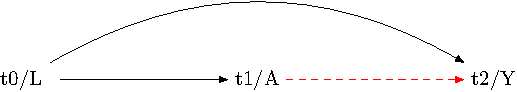
\includegraphics[width=0.8\textwidth,height=\textheight]{use-rev-causal-diagrams_files/figure-pdf/fig-dag-common-cause-1.pdf}

}

\caption{\label{fig-dag-common-cause}Confounding by a common cause. The
red path indicates bias from the open backdoor path from A to Y.}

\end{figure}

\subsubsection{\texorpdfstring{Advice: condition on
\(L\).}{Advice: condition on L.}}\label{advice-condition-on-l.}

To address confounding by a common cause, we should adjust for it by
blocking the backdoor path from the exposure to the outcome. Such
adjustment will restore balance across the levels of \(A\) in the
distribution of confounders that might affect the potential outcomes
\(Y(a*), Y(a)\) under different levels of \(Y(a)\). Again, standard
methods for this adjustment include regression, matching, inverse
probability of treatment weighting, classical G-methods
(\citeproc{ref-hernan2023}{Hernan and Robins 2023}), and more recent
targeted learning frameworks (\citeproc{ref-hoffman2023}{Hoffman
\emph{et al.} 2023}).

Figure~\ref{fig-dag-common-cause-solution} quickly reveals what is
needed:

\begin{enumerate}
\def\labelenumi{\arabic{enumi}.}
\tightlist
\item
  Ensure \(A\) occurs before \(Y\).
\item
  Ensure \(L\) occurs before \(Y\).
\item
  Condition on \(L\).
\end{enumerate}

After time-indexing the nodes on the graph, it becomes evident that
control of confounding generally requires accurate time-series data. Our
chronologically ordered causal diagram serves as a warning for causal
inferences in settings where researchers lack accurately well-recorded
time series data. For example, we often cannot ensure against \(Y\to A\)
or \(Y \to L\) with cross-sectional data.

\begin{figure}

{\centering 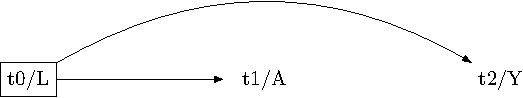
\includegraphics[width=0.8\textwidth,height=\textheight]{use-rev-causal-diagrams_files/figure-pdf/fig-dag-common-cause-solution-1.pdf}

}

\caption{\label{fig-dag-common-cause-solution}Solution: adjust for
pre-exposure confounder. The implication: obtain time series data that
ensure confounders occur before the exposure.}

\end{figure}

\subsubsection{2. The elemental confounding from conditioning on a
mediator}\label{the-elemental-confounding-from-conditioning-on-a-mediator}

If we condition on \(L\) and it forms part of the causal pathway linking
the treatment and the outcome, conditioning on \(L\) may bias the effect
of \(A\) on \(Y\). Here, we focus on \emph{mediator bias}.

Take `beliefs in Big Gods' to be the treatment \(A_{t0}\), `Social
Complexity' to be the outcome \(Y_{t2}\), and `economic trade' to be the
stratified mediator \(L_{t1}\).

In this example, beliefs in Big Gods \(A_{t0}\) directly influence
economic trade \(L_{t1}\), which then affects social complexity
\(Y_{t2}\). Conditioning on economic trade \(L_{t1}\) will downwardly
bias estimates of the total effect of beliefs in Big Gods \(A\) on
social complexity \(Y_{t2}\). Figure~\ref{fig-dag-mediator} presents
this problem.

\begin{figure}

{\centering 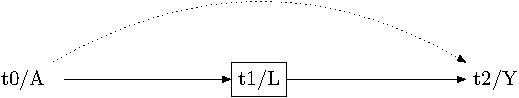
\includegraphics[width=0.8\textwidth,height=\textheight]{use-rev-causal-diagrams_files/figure-pdf/fig-dag-mediator-1.pdf}

}

\caption{\label{fig-dag-mediator}Confounding by conditioning on a
mediator. The dashed red arrow indicates bias arising from partially
blocking the path between A and Y. Here, a true effect of A on Y is
attenuated.}

\end{figure}

\subsubsection{\texorpdfstring{Advice: do not condition on the mediator
by ensuring \(L\) occurs before
\(A\)}{Advice: do not condition on the mediator by ensuring L occurs before A}}\label{advice-do-not-condition-on-the-mediator-by-ensuring-l-occurs-before-a}

Figure~\ref{fig-dag-common-effect-solution-2} presents the solution. We
have encountered the solution before. To avoid mediator bias:

\begin{enumerate}
\def\labelenumi{\arabic{enumi}.}
\tightlist
\item
  Ensure \(A\) occurs before \(Y\).
\item
  Ensure \(L\) occurs before \(Y\).
\item
  Condition on \(L\).
\end{enumerate}

Our chronologically ordered causal diagram shows demands on data
collection and integrity. If we are interested in estimating the total
effect of \(A\to Y\), we must ensure we have measured the relative
timing in the occurrences of \(L\), \(A\), and \(Y\).

\begin{figure}

{\centering \includegraphics[width=0.8\textwidth,height=\textheight]{use-rev-causal-diagrams_files/figure-pdf/fig-dag-common-effect-solution-2-1.pdf}

}

\caption{\label{fig-dag-common-effect-solution-2}Solution: we avoid
mediator bias by ensuring the correct temporal measurement of the
confounder. Here, we draw the black path between A and Y, because we
wish to ensure that this path is unbiased if there is a true causal
effect of A and Y.}

\end{figure}

\subsubsection{3. The elemental confounding from conditioning on a
common effect (collider
stratification)}\label{the-elemental-confounding-from-conditioning-on-a-common-effect-collider-stratification}

\textbf{Case when the collider is a common effect of the exposure and
outcome}

Consider a scenario in which a variable \(L\) is affected by the
treatment \(A\) and outcome \(Y\) (\citeproc{ref-cole2010}{Cole \emph{et
al.} 2010}). According to the rules of d-separation, conditioning on a
common effect, \(L\), will open a non-causal association between \(A\)
and \(Y\).\footnote{In mathematical terms, when \(A\) and \(Y\) are
  independent, their joint probability should equal the product of their
  individual probabilities: \(P(A, Y) = P(A)P(Y)\). However,
  conditioning on \(L\) alters this relationship. The joint probability
  of \(A\) and \(Y\) given \(L\), \(P(A, Y | L)\), does not equal the
  product of \(P(A | L)\) and \(P(Y | L)\). Thus, the common effect
  \(L\) creates an apparent association between \(A\) and \(Y\), which
  is not causal.}

\begin{figure}

{\centering 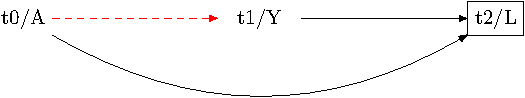
\includegraphics[width=0.8\textwidth,height=\textheight]{use-rev-causal-diagrams_files/figure-pdf/fig-dag-common-effect-1.pdf}

}

\caption{\label{fig-dag-common-effect}Confounding by conditioning on a
collider. The red path indicates bias from the open backdoor path from A
to Y.}

\end{figure}

\subsubsection{\texorpdfstring{Advice: do not condition on a common
effect. Ensure \(L\) occurs before
\(A\).}{Advice: do not condition on a common effect. Ensure L occurs before A.}}\label{advice-do-not-condition-on-a-common-effect.-ensure-l-occurs-before-a.}

We have encountered the solution to this problem before. To avoid
collider bias:

\begin{enumerate}
\def\labelenumi{\arabic{enumi}.}
\tightlist
\item
  Ensure \(A\) occurs before \(Y\).
\item
  Ensure \(L\) occurs before \(Y\).
\item
  Condition on \(L\).
\end{enumerate}

Figure~\ref{fig-dag-common-effect-solution-3} repeats the previous
solutions given in Figure~\ref{fig-dag-common-cause-solution},
Figure~\ref{fig-dag-common-effect}, and
Figure~\ref{fig-dag-common-effect-solution-2}. We are again directed to
demands for ensuring the relative timing in the occurrence of the
variables we need to model. To quantitatively model causality, we must
accurately locate the relative occurrence of \(L\), \(A\), and \(Y\) in
time.

\begin{figure}

{\centering \includegraphics[width=0.8\textwidth,height=\textheight]{use-rev-causal-diagrams_files/figure-pdf/fig-dag-common-effect-solution-3-1.pdf}

}

\caption{\label{fig-dag-common-effect-solution-3}Solution: we ensure
that A and Y are d-separated by ensuring L occurs before A occurs.}

\end{figure}

\textbf{Case when the collider is the effect of exposure}

We have considered how mediator bias may attenuate the total effect
estimate of \(A\) on \(Y\). However, we should not imagine that
conditioning on the effect of an exposure will always bias effect
estimates downward. Consider a scenario in which \(L\) is affected by
both the exposure \(A\) and an unmeasured variable \(U\) related to the
outcome \(Y\) but not to \(A\). Assume that there is no causal effect of
\(A\) on \(Y\). In this scenario, conditioning on \(L\) introduces bias
by opening a backdoor path between \(A\) and \(Y\).
Figure~\ref{fig-dag-descendent} presents these paths, coloured in red.

\begin{figure}

{\centering 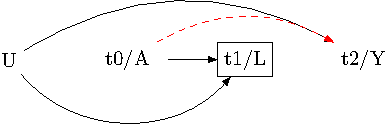
\includegraphics[width=0.8\textwidth,height=\textheight]{use-rev-causal-diagrams_files/figure-pdf/fig-dag-descendent-1.pdf}

}

\caption{\label{fig-dag-descendent}Confounding by descent: the red path
illustrates the biasing path introduced by conditioning on the
descendant of a confounder U that is affected by the exposure, opening a
backdoor path between A and Y.}

\end{figure}

Figure~\ref{fig-dag-descendent} shows the setting of post-exposure
\emph{collider bias}. Conditioning on the collider \(L_{t1}\) in the
analysis induces a non-causal association between \(A_{t0}\) and
\(Y_{t2}\).

\subsubsection{\texorpdfstring{Advice: do not condition on a common
effect. Rather, ensure \(L\) occurs before
\(A\)}{Advice: do not condition on a common effect. Rather, ensure L occurs before A}}\label{advice-do-not-condition-on-a-common-effect.-rather-ensure-l-occurs-before-a}

The strategy builds on the strategy presented in
Figure~\ref{fig-dag-common-cause-solution},
Figure~\ref{fig-dag-common-effect}, and
Figure~\ref{fig-dag-common-effect-solution-2} and
Figure~\ref{fig-dag-common-effect-solution-3}. We will not present it
again:

\begin{enumerate}
\def\labelenumi{\arabic{enumi}.}
\tightlist
\item
  Ensure \(A\) occurs before \(Y\).
\item
  Ensure \(L\) occurs before \(Y\).
\item
  Condition on \(L\) to block the effect of the unmeasured confounder
  \(U\) on \(A\) and \(Y\)
\end{enumerate}

\begin{figure}

{\centering 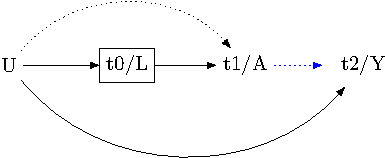
\includegraphics[width=0.8\textwidth,height=\textheight]{use-rev-causal-diagrams_files/figure-pdf/fig-dag-descendent-solution-1.pdf}

}

\caption{\label{fig-dag-descendent-solution}Confounding by descent: the
red path illustrates the biasing path introduced by conditioning on the
descendant of a confounder U that is affected by the exposure, opening a
backdoor path between A and Y.}

\end{figure}

\paragraph{Case of conditioning on a pre-exposure collider
(M-bias)}\label{case-of-conditioning-on-a-pre-exposure-collider-m-bias}

\begin{figure}

{\centering 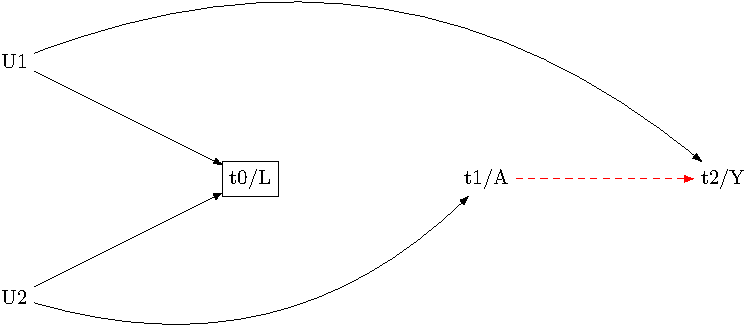
\includegraphics[width=0.8\textwidth,height=\textheight]{use-rev-causal-diagrams_files/figure-pdf/fig-m-bias-1.pdf}

}

\caption{\label{fig-m-bias}M-bias: Confounding control by including
previous outcome measures. The dashed red path indicates bias from the
open backdoor path from A to Y by conditioning on pre-exposure variable
L. The problem arises because L is a collider of unmeasured confounders
U1 and U2, and conditioning on L opens a path from A to U2 to U1 (by
conditioning on L) to Y. This path is shown in red.}

\end{figure}

One must be cautious not to over-condition on pre-exposure variables. In
settings where we condition on a variable that is itself not associated
with the exposure or outcome but is the descendent of an unmeasured
instrumental variable as well as of an unmeasured cause of the outcome,
we may inadvertently induce confounding known as `M-bias', illustrated
in Figure~\ref{fig-m-bias},

M-bias can arise even though a variable \(L\) that induces it occurs
before the treatment \(A\). Conditioning on \(L\) creates a spurious
association between \(A\) and \(Y\) by opening the path between the
unmeasured confounders. We assume that \(A\) and \(Y\) might be
unconditionally independent (\(A \coprod Y(a)\)). However, when
stratified by \(L\), this independence is violated:
(\(A \cancel{\coprod} Y(a)| L\)). This form of bias is another
manifestation of collider stratification bias. This manifestation
pertains to conditioning on pre-exposure variables in certain structural
scenarios.\footnote{When the path is ordered chronologically from left
  to right, the ``M'' shape, giving M-bias its name, changes to an ``E''
  shape. However, the term ``M-bias'' is retained.}

\subsubsection{Advice: avoid the ``causal
salad''}\label{advice-avoid-the-causal-salad}

\begin{figure}

{\centering \includegraphics[width=0.8\textwidth,height=\textheight]{use-rev-causal-diagrams_files/figure-pdf/fig-m-bias-solution-1.pdf}

}

\caption{\label{fig-m-bias-solution}M-bias is avoided when by not
conditioning on pre-exposure variable L. Doing so reveals all open
backdoor paths are blocked. They are blocked because L is a collider of
the unmeasured variables U1 and U2. If we do not condition on L, the
path between U1 and U2 remains closed.}

\end{figure}

Do not adopt an indiscriminate approach to confounding control, what
Richard McElreath aptly calls the ``causal salad''
(\citeproc{ref-mcelreath2020}{McElreath 2020}). Even if we can
accurately measure the occurrence of our variables in time, conditioning
on a pre-exposure variable may induce bias. The best-lights of
subject-matter experts must inform our graphs.

Figure~\ref{fig-m-bias-solution} shows the solution to conditioning on a
pre-exposure collider where doing so evokes M-bias.

\subsubsection{4. Conditioning on a descendant (for good or
bad).}\label{conditioning-on-a-descendant-for-good-or-bad.}

Recall that by conditioning on a descendent, we partially conditioning
on its parents. We next consider a case in which conditioning on a
descendent amplifies bias, followed by a case in which conditioning on a
descendent reduces bias.

\paragraph{Case when conditioning on a descendant amplifies
bias}\label{case-when-conditioning-on-a-descendant-amplifies-bias}

Suppose a team of anthropologists studies the relationship between the
use of a specific social ritual \(A\) and the level of technological
advancement \(Y\) in different human societies.

Let \(U\) represent ancestral language families, which influence the
development of unique social rituals \(A\). For instance, isolated
language families may develop distinct cultural practices. We assume
\(U\) is unmeasured. Now, let \(S\) denote the sample of available
cultures. Here, we consider that \(S\) is affected by language families
in such a way that anthropologists may prefer studying cultures from
certain ancestral language families. This preference leads to a sample
that is representative of only some cultures. Suppose there is no direct
causal link between ancestral language family \(U\) and technological
advancement \(Y\). However, we posit that technologically advanced
societies (\(Y\)) are more likely to be documented due to better
accessibility and more comprehensive documentation. This documentation
bias affects the sample \(S\). We also assume no causal association
exists between \(A\) and \(Y\).

In this scenario, as depicted in Figure~\ref{fig-dag-selection-outcome},
if anthropological studies focus only on societies that have been
extensively studied and documented (\(S\)), we inadvertently condition
on an effect of \(Y\) and an unmeasured confounder \(U\). This
conditioning introduces a non-causal path between the social ritual
\(A\) and technological advancement \(Y\), leading to an instance of
\emph{selection bias}. This bias is particularly problematic because it
arises from the data collection process itself and cannot be resolved by
simply adjusting for measured variables.

By conditioning on \(S\) (extent of study), a spurious association
between the social ritual and technological advancement is introduced.
As a result, we may incorrectly infer a direct link between certain
social rituals and levels of technological development. This observed
correlation could arise because less isolated societies, which are more
likely to be studied, independently develop specific social rituals and
acquire technologies for reasons unrelated to \(A\).

To mitigate this bias, alternative strategies such as collecting a more
diverse and representative sample or using advanced statistical methods
tailored for selection bias are required. It's crucial to approach such
studies with an awareness of these potential biases and to design
research methodologies that can account for or minimize their effects.

\begin{figure}

{\centering \includegraphics[width=0.8\textwidth,height=\textheight]{use-rev-causal-diagrams_files/figure-pdf/fig-dag-selection-outcome-1.pdf}

}

\caption{\label{fig-dag-selection-outcome}Confounding by descendant of
the outcome: the red path illustrates the biasing path introduced by
conditioning on the descendant of a confounder U that is affected by the
outcome Y, leading to a non-causal association of between A and Y. This
is an example of selection bias. It cannot be undone by conditioning. To
remove this bias, we must accurately measure Y.}

\end{figure}

\paragraph{Advice: we cannot address this form of selection bias by
conventional
means}\label{advice-we-cannot-address-this-form-of-selection-bias-by-conventional-means}

We cannot address this form of selection bias through confounding
control. Here, our causal diagram is helpful because it tells us we need
to stop and consider how to recover unbiased measurements of \(Y\).

\paragraph{Case when conditioning on a descendant reduces
bias}\label{case-when-conditioning-on-a-descendant-reduces-bias}

Consider a scenario where adjusting for a post-treatment descendant
variable, denoted as \(L^\prime\), can help mitigate bias. Imagine an
unmeasured confounder \(U\) that influences \(A\), \(Y\), and
\(L^\prime\), with the effect on \(L^\prime\) occurring after both \(A\)
and \(Y\). In this context, adjusting for \(L^\prime\) could lessen the
confounding caused by the unmeasured confounder \(U\). This approach
aligns with the modified disjunctive cause criterion for confounding
control, which suggests including as a covariate any proxy for an
unmeasured variable that is a common cause of both the exposure and the
outcome (\citeproc{ref-vanderweele2019}{VanderWeele 2019}). As
illustrated in Figure~\ref{fig-dag-descendent-solution-2}, although
\(L^\prime\) occurs after the exposure and possibly even after the
outcome, conditioning on it can reduce confounding.

How does this work in practice? For example, consider a genetic factor
that influences both the exposure and the outcome early in life but is
expressed later. Adjusting for this later-life expression of the genetic
factor can help control for the effect of the unmeasured confounding,
which influenced both \(A\) and \(Y\). Even though \(L'\) occurs after
the outcome, conditioning on \(L'\) is sensible strategy because \(L'\)
provides information about \(U\). This example illustrates the prospect
of post-outcome confounding control.
Figure~\ref{fig-dag-descendent-solution-2} presents this desirable form
of post-outcome conditioning.

\begin{figure}

{\centering 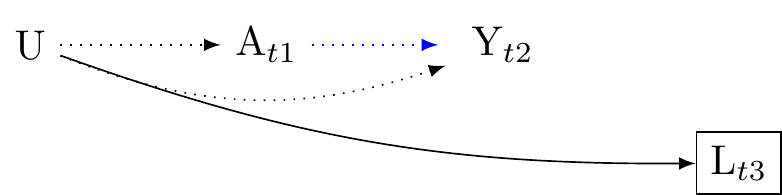
\includegraphics[width=0.8\textwidth,height=\textheight]{use-rev-causal-diagrams_files/figure-pdf/fig-dag-descendent-solution-2-1.pdf}

}

\caption{\label{fig-dag-descendent-solution-2}Solution: Conditioning on
a confounder that occurs after both the exposure and the outcome can
address unmeasured confounding if the confounder is a descendant of a
prior common cause of the exposure and outcome. The red dotted paths
underscore that the effect of U on A and Y is partially adjusted by
conditioning on L', even though L' occurs after the outcome. The paths
are dotted to represent the bias reduction achieved by conditioning on
the post-outcome descendant of an unmeasured common cause of the
exposure and outcome. An example is a genetic factor affecting the
exposure and outcome early in life, which can be measured later in life.
Adjusting for such an indicator is an example of post-outcome
confounding control.}

\end{figure}

\paragraph{Advice: when developing a conditioning set, adopt the
modified disjunctive cause
criterion}\label{advice-when-developing-a-conditioning-set-adopt-the-modified-disjunctive-cause-criterion}

The prospect that we may use descendants for confounding control reveals
that even if for a causal diagram, ``timing is everything,'' when
analysing a problem, \textbf{structure is everything}. Our
chronologically hygienic graph reveals the scope for conditioning on
confounders that occcur after the exposure and outcome occur. It brings
home the point that we should think of the concept of a confounder as
meaningful relative the adjustment set in which it forms a part.

We are now in a position to understand why VanderWeele's modified
disjunctive cause criteria for selecting this confounder set it
desirable. This advice will lead us to remove every instrumental
variable unless it is a descendant of an unmeasured confounder of the
exposure and outcome. Neither U1 nor U2 satisfy this property.

Practically speaking, determining which variables belong in the
confounder set can be challenging. We take instruction from the best
lights of experts. However, science is the practice of revising expert
opinion. We assume experts may be wrong. For this reason, we should
perform sensitivity analyses.

\subsection{Part 3. Interaction, Mediation, and Longitudinal
Feedback}\label{part-3.-interaction-mediation-and-longitudinal-feedback}

We may wish to understand whether how effects vary across
sub-populations or how the joint effect of two interventions differs
from their individual effects or no intervention at all. How shall we
conceive of these interventions and comparisons? How shall we represent
them on a graph?

\subsubsection{Warning: Do not attempt a special graphical presentation
of causal
interactions}\label{warning-do-not-attempt-a-special-graphical-presentation-of-causal-interactions}

When depicting causal interactions on graphs, it is essential to focus
on their primary purpose: examining confounding. It is not the function
of a causal diagram to represent non-linear relationships or
interactions. Instead, they should help us understand whether and how
unbiased estimates may be obtained from data. We should avoid
unnecessary complexities in these diagrams, such as trying to represent
additive or multiplicative interactions visually. Such complexities
distract researchers from a focus on identifying potential sources of
bias. Including nodes and paths should be strictly limited to what is
necessary for assessing the specified causal contrasts.

\subsubsection{A tale of two
interactions}\label{a-tale-of-two-interactions}

The concept of interaction varies based on the causal question at hand.
Here, we consider two distinct approaches to framing questions about
causal interaction:

\paragraph{Approach 1: interaction as a
double-exposure}\label{approach-1-interaction-as-a-double-exposure}

Causal interaction can refer to the combined versus separate effects of
two distinct exposures. We consider evidence of causal interaction at a
given scale when one exposure's effect on an outcome is contingent on
the level of another exposure.

For instance, consider the effect of beliefs in Big Gods (exposure
\(A\)) on social complexity (outcome \(Y\)), potentially influenced by a
culture's monumental architecture (exposure \(B\)). To assess the
individual and combined effects of \(A\) and \(B\), we look for evidence
of causal interaction on the difference scale. Evidence for interaction
is present if the following inequality holds:

\[\bigg(\underbrace{\mathbb{E}[Y(1,1)]}_{\text{joint exposure}} - \underbrace{\mathbb{E}[Y(0,0)]}_{\text{neither exposed}}\bigg) - \bigg[ \bigg(\underbrace{\mathbb{E}[Y(1,0)]}_{\text{only A exposed}} - \underbrace{\mathbb{E}[Y(0,0)]}_{\text{neither exposed}}\bigg) + \bigg(\underbrace{\mathbb{E}[Y(0,1)]}_{\text{only B exposed}} - \underbrace{\mathbb{E}[Y(0,0)]}_{\text{neither exposed}} \bigg)\bigg] \neq 0 \]

This equation simplifies to

\[ \underbrace{\mathbb{E}[Y(1,1)]}_{\text{joint exposure}} - \underbrace{\mathbb{E}[Y(1,0)]}_{\text{only A exposed}} - \underbrace{\mathbb{E}[Y(0,1)]}_{\text{only B exposed}} + \underbrace{\mathbb{E}[Y(0,0)]}_{\text{neither exposed}} \neq 0 \]

A positive value suggests additive interaction. A negative value
suggests sub-additive interaction. A value near zero implies no reliable
evidence for interaction.

It is important to understand that evidence for causal interaction can
differ by the scale one chooses to assess it.{[}\^{}11{]}

{[}\^{}11{]} Causal effect estimates for interaction give different
interpretations when measured on the ratio scale. This discrepancy can
have significant policy implications, see:
(\citeproc{ref-vanderweele2014}{VanderWeele and Knol 2014}). Although
beyond the scope of this article, it is worth emphasising again that
when evaluating evidence for causality, in addition to specifying the
exposure and outcome, we must specify the measure of effect in which we
are interested, as well as the target population for whom we wish to
generalise (\citeproc{ref-hernuxe1n2004}{Hernán 2004};
\citeproc{ref-tripepi2007}{Tripepi \emph{et al.} 2007}).

Lastly, causal diagrams, being non-parametric, do not directly represent
interactions. However, they can suggest the presence of an interaction
by showing two exposures jointly influencing an outcome while
maintaining their independence. Figure Figure~\ref{fig-dag-interaction}
illustrates this concept.{[}\^{}11{]}

\begin{figure}

{\centering 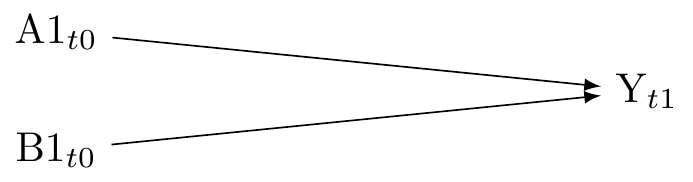
\includegraphics[width=0.6\textwidth,height=\textheight]{use-rev-causal-diagrams_files/figure-pdf/fig-dag-interaction-1.pdf}

}

\caption{\label{fig-dag-interaction}Causal Diagram Illustrating
Interaction: This diagram represents the individual and joint effects of
two exposures, A and B, on outcome Y. We assume that A and B are
causally independent. The diagram includes confounders L1 and L2, which
are necessary for controlling backdoor paths related to both exposures.
The counterfactual outcome is Y(a,b), and evidence for additive or
subadditive interaction is indicated if E{[}Y(1,1) - Y(0,1) - Y(1,0) +
Y(0,0){]} ≠ 0. If B cannot be conceptualised as a variable amenable to
intervention, we may focus on effect modification but not interaction.
Note: paths should be distinct and not intersect each other.}

\end{figure}

Note that the chronological order in Figure~\ref{fig-dag-interaction}
reveals demands on data collection. Ensuring that \(A\) and \(B\) do not
affect each other requires (1) expert knowledge about \(A\) and \(B\)
(2) measurements of \(A\) and \(B\) at intervals in which there can be
no directed effects.

\paragraph{Approach 2: interaction as effect-modification under a single
exposure}\label{approach-2-interaction-as-effect-modification-under-a-single-exposure}

Effect modification analysis seeks to understand how the effect of an
exposure varies across different strata of another variable or in more
complex cases, across strata of multiple variables. A stratum where the
exposure's effect differs is termed an `effect modifier.'

For example, consider again a study assessing the causal effect of
beliefs in Big Gods on social complexity. Suppose we are interested in
whether this effect varies by region, geography becomes our `effect
modifier.' Imagine contrasting North American societies with Continental
societies. Here, we do not treat geography as an intervention--- it is
conceptually implausible to do so. Instead, we investigate whether
geography modifies the effect of a defined exposure (beliefs in Big
Gods) on a specific outcome (social complexity).

\[\hat{E}[Y(a)|G=g]\]

This quantity represents the expected outcome under exposure \(a\) for
group \(g\).

Similarly, the expected outcome for exposure level \(A = a^*\) among
individuals in the same group (\(G = g\)) is expressed:

\[\hat{E}[Y(a^*)|G=g]\]

The causal effect of shifting the exposure level from \(a^*\) to \(a\)
within group \(g\) is thus expressed:

\[\hat{\delta}_g = \hat{E}[Y(a)|G=g] - \hat{E}[Y(a^*)|G=g]\]

The quantity on the left computes the change in the expected outcome
from altering the exposure from \(a^*\) to \(a\) within group \(g\).

Likewise, the causal effect of changing the exposure from \(a^*\) to
\(a\) within group \(g'\) is expressed:

\[\hat{\delta}_{g'} = \hat{E}[Y(a)|G=g'] - \hat{E}[Y(a^*)|G=g']\]

Here, \(\hat{\delta}_{g'}\) captures the analogous effect of the
exposure within group \(g'\).

To understand effect modification, we compare the conditional causal
effect estimate on a difference scale between these two groups, which we
calculate as:

\[\hat{\gamma} = \hat{\delta}_g - \hat{\delta}_{g'}\]

The value of \(\hat{\gamma}\) quantifies the differential effect of
shifting the exposure from \(a^*\) to \(a\) between groups \(g\) and
\(g'\). \(\hat{\gamma} \neq 0\) would suggest variability in the effect
of the exposure based on group characteristics.\footnote{For
  distinctions within varieties of effect modification relevant to
  strategies of confounding control, see
  (\citeproc{ref-vanderweele2007}{VanderWeele and Robins 2007}).}

\begin{figure}

{\centering 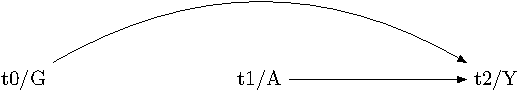
\includegraphics[width=0.8\textwidth,height=\textheight]{use-rev-causal-diagrams_files/figure-pdf/fig-dag-effect-modfication-1.pdf}

}

\caption{\label{fig-dag-effect-modfication}A simple graph depicting
effect-modification in which there are no confounders. G is an effect
modifier of A on Y. We draw a box around G to indicate we are
conditioning on this variable.}

\end{figure}

\subsubsection{Causal Mediation: The limitations of standard
approaches}\label{causal-mediation-the-limitations-of-standard-approaches}

In the human sciences, mediation analysis is often mired in confusion, a
situation exacerbated by the complex nature of causal relationships it
aims to reveal. Beyond the intrinsic challenges of mediation analysis,
much of the prevailing confusion stems from the prevalent use of
structural equation models (SEMs). These models generally lack a
systematic way of conceiving and modelling the counterfactual contrasts,
that are relevant to evaluating causality. In most cases is unclear what
SEM (so-called structural equation modelling) delivers. Attempts at
mediation using regression generally do no better
(\citeproc{ref-vanderweele2015}{VanderWeele 2015}). This disconnect
between the modelling tradition and the demands of causal data science
produces statistic models that are conceptually adrift from the causal
structures they intend to represent. Lacking a clear conceptual
framework to assess the relevant structural relationships, traditional
approaches frequently yield ambiguous and scientifically questionable
results. The counterfactual framework of causal data science allows us
to do better. And so we should.

\paragraph{Defining the estimands}\label{defining-the-estimands}

To gain a clearer understanding of what causal mediation entails, it is
helpful to decompose the total effect into the natural direct and
indirect effects.

The total effect of treatment \(A\) on outcome \(Y\) is defined as the
aggregate difference between the potential outcomes when the treatment
is applied versus when it is not. The estimand for the total effect (TE)
can be expressed as follows:

\[
\Delta_{ATE} = TE = Y(1) - Y(0)
\]

This total effect can further decomposed into direct and indirect
effects, which allow us to address questions of mediation.

The potential outcome \(Y(1)\) can be stated:

\[ 
Y(1) = Y(1, M(1))
\]

Here, the effect of the exposure, set to \(A = 1\), is considered along
with the effect of the mediator at its natural value when \(A = 1\)

Similarly, the potential outcome \(Y(0)\) can be stated:

\[ 
Y(0) = Y(0, M(0))
\]

This gives us the effect when the exposure is inactive, \(A = 0\), with
the mediator taking its natural value in this scenario.

Now, let us use these components to explicate mediated causal effects:

\textbf{Natural Direct Effect (NDE):} is the effect of the treatment on
the outcome while maintaining the mediator at the level it would have
been if the treatment had \emph{not} been applied. The always-unobserved
portion of this counterfactual quantity is highlighted in blue for
emphasis.

The NDE is expressed as:

\[
 NDE = \textcolor{blue}{Y(1, M(0))} - Y(0, M(0))
 \]

\textbf{Natural Indirect Effect (NIE):} This reflects the portion of the
treatment's effect on the outcome that is mediated. It compares the
potential outcome under treatment (where the mediator assumes its
natural level under treatment) with the potential outcome where the
mediator assumes its natural value under no treatment. This part of the
counterfactual quantity is highlighted in blue; it is the same quantity
previously highlighted in blue, and is never directly observed.

The NIE is expressed as:

\[
 NIE = Y(1, M(1)) - \textcolor{blue}{Y(1, M(0))}
\]

By rearranging this decomposition, we can demonstrate that the total
effect (TE) is the sum of the NDE and NIE. To achieve this, we add and
subtract the term \(\textcolor{blue}{Y(1, M(0))}\), highlighted in blue:

\[
TE = NDE + NIE = [Y(1, M(1)) - \textcolor{blue}{Y(1, M(0))}] + [\textcolor{blue}{Y(1, M(0))} - Y(0, M(0))]
\]

This decomposition of the total effect into natural direct and indirect
effects explicates the set of estimands we typically seek causal
mediation analysis. To express these quantities requires conceptualising
them in relation to counterfactuals. Lacking these estimands it is
unclear what we are estimating when performing mediation analyses.
Contrary to their name, structural equation models typically lack an
inherent structural basis for interpretation. They would be aptly
described as `un-structural equation models.'

Approaching mediation from a structural perspective, as enabled by
causal data science, allows for the decomposition of the Total Effect
into parts mediated by changes in the mediator arising from the
treatment (NIE) and those that are unmediated (NDE). Only with these
targeted counterfactual contrasts in mind can we effectively address
causal mediation questions and draw valid inferences. Furthermore, we
need these statements to evaluate sources of confounding.
Chronologically ordered causal diagrams help assess the stringent
demands for satisfying assumptions of `no unmeasured confounding' in
this setting.

\subsubsection{Chronological Causal Diagrams in Causal Mediation
Analysis}\label{chronological-causal-diagrams-in-causal-mediation-analysis}

Consider again the hypothesis that cultural beliefs in `Big Gods'
influence social complexity, with political authority serving as a
mediator. Let's assume these broad concepts are well-defined. What
requirements are necessary to answer this hypothesis?

\begin{enumerate}
\def\labelenumi{\arabic{enumi}.}
\tightlist
\item
  \textbf{No Unmeasured Exposure-Outcome Confounder}
\end{enumerate}

This requirement is expressed: \(Y(a,m) \coprod A | L1\). After
accounting for the covariates in set \(L1\), there must be no unmeasured
confounders influencing cultural beliefs in Big Gods (\(A\)) and social
complexity (\(Y\)). For example, if our study examines the causal effect
of cultural beliefs in Big Gods (the exposure) on social complexity (the
outcome), and the covariates in \(L1\) include factors like geographic
location and historical context, we need to ensure that these covariates
effectively block any confounding paths between \(A\) and \(Y\).
Figure~\ref{fig-dag-mediation-assumptions} shows this confounding path
in brown.

\begin{enumerate}
\def\labelenumi{\arabic{enumi}.}
\setcounter{enumi}{1}
\tightlist
\item
  \textbf{No unmeasured mediator-outcome confounder}
\end{enumerate}

This requirement is expressed: \(Y(a,m) \coprod M | L2\). After
controlling for the covariate set \(L2\), we must ensure that no other
unmeasured confounders affect the political authority \(M\) and social
complexity \(Y\). For instance, if trade networks impact political
authority and social complexity, to obstruct the unblocked path linking
our mediator and outcome we must account for trade networks.
Furthermore, we must be entitled to assume the absence of any other
confounders for the mediator-outcome path.
Figure~\ref{fig-dag-mediation-assumptions} shows this confounding path
is represented in blue.

\begin{enumerate}
\def\labelenumi{\arabic{enumi}.}
\setcounter{enumi}{2}
\tightlist
\item
  \textbf{No unmeasured exposure-mediator confounder}
\end{enumerate}

This requirement is expressed: \(M(a) \coprod A | L3\). After
controlling for the covariate set \(L3\), we must ensure that no
additional unmeasured confounders affect cultural beliefs in Big Gods
\(A\) and political authority \(M\). For example, the capability to
construct large ritual theatres may influence the belief in Big Gods and
the level of political authority. If we have indicators for this
technology measured prior to the emergence of Big Gods (these indicators
being \(L3\)), we must assume that accounting for \(L3\) closes the
backdoor path between the exposure and the mediator.
Figure~\ref{fig-dag-mediation-assumptions} shows this confounding path
in green.

\begin{enumerate}
\def\labelenumi{\arabic{enumi}.}
\setcounter{enumi}{3}
\tightlist
\item
  \textbf{No mediator-outcome confounder affected by the exposure}
\end{enumerate}

This requirement is expressed: \(Y(a,m) \coprod M(a^*) | L\). We must
ensure that no variables confounding the relationship between political
authority and social complexity in \(L2\) are themselves influenced by
the cultural beliefs in Big Gods (\(A\)). For example, when studying the
effect of cultural beliefs in Big Gods (\(A\), the exposure) on social
complexity (\(Y\), the outcome) as mediated by political authority
(mediator), there can be no factors, such as trade networks (\(L2\)),
that influence both political authority and social complexity and are
affected by the belief in Big Gods.
Figure~\ref{fig-dag-mediation-assumptions} shows this confounding path
in red.

\textbf{Note: the assumption of no exposure-induced confounding in the
mediator-outcome relationship is often a substantial obstacle for causal
mediation analysis.} Where the exposure influences a confounder of the
mediator and outcome, we face a dilemma. Without accounting for this
confounder, a backdoor path between the mediator and the outcome would
remain open. However, by accounting for it, we partially obstruct the
path between the exposure and the mediator, leading to bias. In this
setting, we cannot recover the natural direct and indirect effects
directly from any observational data
(\citeproc{ref-vanderweele2015}{VanderWeele 2015}).

Notice again that the requirements for counterfactual data analysis are
considerably stricter than has been appreciated in the structural
equation modelling traditions. Unfortunately, a generation of
researchers must unlearn the habit of leaping from a description of a
statistical process as embodied in a structural equation diagram to the
analysis of the data. It has been over three decades since Robins and
Greenland demonstrated that we cannot understand the quantities we are
estimating in mediation analysis without first specifying the estimands
of interest in terms of the targeted counterfactuals of interest
(\citeproc{ref-robins1992}{Robins and Greenland 1992}). Moreover, where
the Natural Direct and Indirect Effects are of interest, such estimands
require conceptualising a rather unusual counterfactual that is
\emph{never} directly observed from the data, namely:
\(\textcolor{blue}{Y(1, M(0))}\), and, only after stringent assumptions
are satisfied, simulating it from data (for an extensive discussion,
see:VanderWeele (\citeproc{ref-vanderweele2015}{2015})).

\begin{figure}

{\centering \includegraphics[width=1\textwidth,height=\textheight]{use-rev-causal-diagrams_files/figure-pdf/fig-dag-mediation-assumptions-1.pdf}

}

\caption{\label{fig-dag-mediation-assumptions}This causal diagram
illustrates the four fundamental assumptions needed for causal mediation
analysis. The first assumption pertains to the brown paths. It requires
the absence of an unmeasured exposure-outcome confounder, and assumes
that conditioning on L1 is sufficient for such confounding control. The
second assumption pertains to the blue paths. It requires the absence of
an unmeasured mediator-outcome confounder and assumes that conditioning
on L2 is sufficient for such confounding control. The third assumption
pertains to the green paths. It requires the absence of an unmeasured
exposure-mediator confounder and assumes that conditioning on L3 is
sufficient for such confounding control. The fourth and final assumption
pertains to the red paths. It requires the absence of a mediator-outcome
confounder that is affected by the exposure and assumes that there is no
path from the exposure to L2 to M. If the exposure were to affect L2,
then conditioning on L2 would block the exposure's effect on the
mediator, as indicated by dashed red path. Causal diagrams not only
clarify how different types of confounding bias may converge (here
mediation bias and confounder bias), but also reveal the limitations of
common methods such as structural equation models and multi-level models
for handling time-series data where the fourth assumption fails -- that
is, where there is treatment-confounder feedback. Such feedback is
common in time-series data, but not widely understood. For example,
structural equation models and multi-level models cannot address causal
questions in the presence of such feedback, but these models remain
widely favoured.}

\end{figure}

\subsubsection{Case 3: Longitudinal
Feedback}\label{case-3-longitudinal-feedback}

Our discussion of causal mediation primarily focused on how effects from
two sequential exposures may combine to influence an outcome. This
concept can be expanded to investigate the causal effects of multiple
sequential exposures. In such cases, researchers often gravitate towards
longitudinal growth models. However, a critical question arises: Where
do counterfactuals fit within these models? Without incorporating
counterfactuals, the conclusions we derive become questionable.
Chronologically ordered causal diagrams can be instrumental in
highlighting the challenges and opportunities in these scenarios.

For instance, let us consider multiple exposures fixed in time. There
are four distinct counterfactual outcomes, each corresponding to a fixed
treatment regime:

\begin{enumerate}
\def\labelenumi{\arabic{enumi}.}
\tightlist
\item
  \textbf{Always Treat (Y(1,1))}
\item
  \textbf{Never Treat (Y(0,0))}
\item
  \textbf{Treat Once First (Y(1,0))}
\item
  \textbf{Treat Once Second (Y(0,1))}
\end{enumerate}

\phantomsection\label{tbl-regimes}
\begin{longtable}[]{@{}
  >{\raggedright\arraybackslash}p{(\columnwidth - 4\tabcolsep) * \real{0.1351}}
  >{\raggedright\arraybackslash}p{(\columnwidth - 4\tabcolsep) * \real{0.5405}}
  >{\raggedright\arraybackslash}p{(\columnwidth - 4\tabcolsep) * \real{0.3243}}@{}}
\caption{\label{tbl-regimes}Table outlines four fixed treatment regimes
and six causal contrasts in time-series data where exposure
varies.}\tabularnewline
\toprule\noalign{}
\begin{minipage}[b]{\linewidth}\raggedright
Type
\end{minipage} & \begin{minipage}[b]{\linewidth}\raggedright
Description
\end{minipage} & \begin{minipage}[b]{\linewidth}\raggedright
Counterfactual Outcome
\end{minipage} \\
\midrule\noalign{}
\endfirsthead
\toprule\noalign{}
\begin{minipage}[b]{\linewidth}\raggedright
Type
\end{minipage} & \begin{minipage}[b]{\linewidth}\raggedright
Description
\end{minipage} & \begin{minipage}[b]{\linewidth}\raggedright
Counterfactual Outcome
\end{minipage} \\
\midrule\noalign{}
\endhead
\bottomrule\noalign{}
\endlastfoot
Regime & Always treat & Y(1,1) \\
Regime & Never treat & Y(0,0) \\
Regime & Treat once first & Y(1,0) \\
Regime & Treat once second & Y(0,1) \\
Contrast & Always treat vs.~Never treat & E{[}Y(1,1) - Y(0,0){]} \\
Contrast & Always treat vs.~Treat once first & E{[}Y(1,1) - Y(1,0){]} \\
Contrast & Always treat vs.~Treat once second & E{[}Y(1,1) -
Y(0,1){]} \\
Contrast & Never treat vs.~Treat once first & E{[}Y(0,0) - Y(1,0){]} \\
Contrast & Never treat vs.~Treat once second & E{[}Y(0,0) - Y(0,1){]} \\
Contrast & Treat once first vs.~Treat once second & E{[}Y(1,0) -
Y(0,1){]} \\
\end{longtable}

We can compute six causal contrasts for these four fixed regimes, as
shown in Table~\ref{tbl-regimes}.\footnote{The number of possible
  contrast combinations can be calculated as
  \(C(n, r) = \frac{n!}{(n-r)! \cdot r!}\)}

Treatment assignments may be modelled as conditional shift functions of
previous outcomes, a concept known as ``time-varying treatment
regimes.'' Comparisons between relevant counterfactual quantities are
necessary to estimate the causal effects of time-varying treatment
regimes. In mediation analysis time-varying confounding was a concern
(recall condition 4: exposure must not affect mediator/outcome
confounders). This principle of confounding control applies to
sequential time-varying treatments. Unlike traditional causal mediation
analysis, however, we might be interested in treatment sequences over
extended periods, i.e.~\(Y(00011)\) contrasted with \(Y(00000)\). Which
estimand we consider should depend on the context of our scientific
question.

Chronological causal diagrams are valuable tools for identifying
problems with traditional multi-level regression analysis and structural
equation modelling. For example, let us examine the impact of belief in
Big Gods on social complexity. Start by estimating a fixed treatment
regime. Assume we have well-defined concepts of Big Gods and social
complexity, and assume we have accurate measurements over time. Suppose
we assess the effects of beliefs in Big Gods on a well-defined,
well-measured measure of social complexity two centuries after a shift
to big-Gods has occurred.

Fixed treatment strategies include comparing ``always believing in big
Gods'' versus ``never believing in big Gods'' and their effects on
social complexity conceived as a counterfactual contrast across
conditionally exchangeable groups of `treated' and `untreated'
societies. Refer to Figure~\ref{fig-dag-9}. Here, \(A_{tx}\) represents
the belief in Big Gods at time \(tx\), and \(Y_{tx}\) denotes the
outcome, social complexity, at time \(x\). Imagine economic trade,
represented as \(L_{tx}\), is a time-varying confounder with changing
effects over time, influencing economic trade. An unmeasured confounder,
\(U\), such as oral traditions, might also influence belief in Big Gods
and social complexity.

In a scenario where we can reasonably infer that the level of economic
trade at time \(0\) (\(L_{t0}\)) impacts beliefs in Big Gods at time
\(1\) (\(A_{t1}\)), we draw an arrow from \(L_{t0}\) to \(A_{t1}\).
Conversely, if belief in Big Gods at time \(1\) (\(A_{t1}\)) affects
future levels of economic trade (\(L_{t2}\)), an arrow from \(A_{t1}\)
to \(L_{t2}\) is warranted. This causal diagram demonstrates a feedback
process between the time-varying exposure \(A\) and the time-varying
confounder \(L\). Figure~\ref{fig-dag-9} displays this
exposure-confounder feedback loop. In practical scenarios, the diagram
might include more arrows, but our goal here is to illustrate the issue
of exposure-confounder feedback with the minimal necessary arrows.

What if we were to condition on the time-varying confounder \(L_{t3}\)?
To consequences emerge: first, we block all backdoor paths between the
exposure \(A_{t2}\) and the outcome \(Y\), which is crucial for
eliminating confounding. This result of our confounding strategy is
positive: we exert confounding control. However, this conditioning also
closes previously open paths, introducing structural sources of bias.
For example, the path \(A_{t1}, L_{t2}, U, Y_{t4}\), previously open,
would now be activated as the time-varying confounder becomes a common
effect of \(A_{t1}\) and \(U\). This result of our confounding strategy
is negative: we lose confounding control. Conditioning on a time-varying
confounder is a double-edged sword: essential for blocking backdoor
paths but potentially opening other problematic pathways. This conundrum
when conditioning on a confounder affected by prior exposure ---being
damned if we do, damned if we don't --- is a critical consideration in
longitudinal feedback analysis. We may assume it to be the rule, rather
than the exception.

\begin{figure}

{\centering 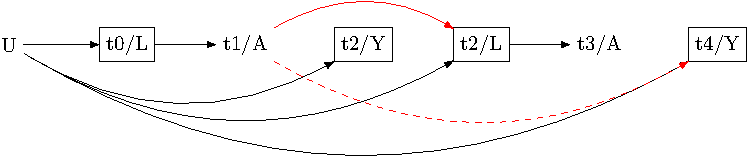
\includegraphics[width=1\textwidth,height=\textheight]{use-rev-causal-diagrams_files/figure-pdf/fig-dag-9-1.pdf}

}

\caption{\label{fig-dag-9}Exposure confounder feedback is a problem for
time-series models. If we do not condition on L\_t2, a backdoor path is
open from A\_t3 to Y\_t4. However, if conditioning on L\_t2 introduces
collider bias, opening a path, coloured in red, between A\_t2 and Y\_t4.
Here, we may not use conventional methods to estimate the effects of
multiple exposures. Instead, at best, we may obtain controlled effects
using special methods, such G-methods, TMLE, SDR and others. Multi-level
models will not eliminate bias here.}

\end{figure}

There is scope for time varying confounding in the absence of
treatment-confounder feedback. When a time-varying exposure and a
time-varying confounder share a common cause, even in cases where the
exposure does not directly influence the confounder, a backdoor path is
opened because the time-varying confounder is a common effect of two
unmeasured confounders, one of which affects the previous exposure.
Figure~\ref{fig-dag-time-vary-common-cause-A1-l1} presents this
scenario. Standard methods cannot such as regression and structural
equation modelling (SEM) cannot recover unbiased causal effects.

\begin{figure}

{\centering 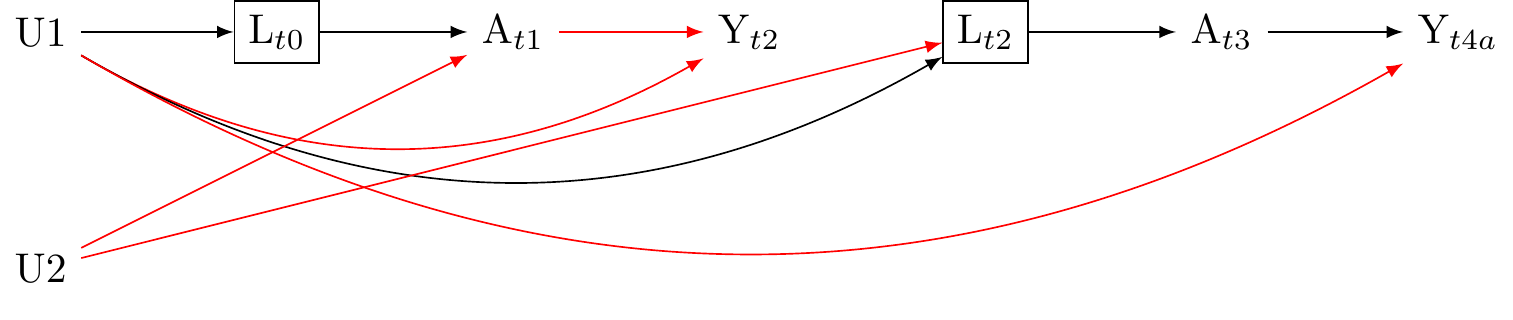
\includegraphics[width=1\textwidth,height=\textheight]{use-rev-causal-diagrams_files/figure-pdf/fig-dag-time-vary-common-cause-A1-l1-1.pdf}

}

\caption{\label{fig-dag-time-vary-common-cause-A1-l1}Exposure confounder
feedback is a problem for time-series models. Here, we do not assume
that A\_t1 affects L\_t2. However, if an unmeasured variable (U\_2)
affects both the exposure A\_t1 and the cofounder L\_2, an unblocked
path opens, linking exposure to outcome (shown in red). Again, we cannot
infer causal effects using regression-based methods: if we are
`damed-if-we-do-damned-if-we-do-not' condition on L\_t2. In this
setting, to address causal questions, we require simulation-based
estimators.}

\end{figure}

The issue of treatment confounder feedback poses significant challenges
in evolutionary human science. Again, this problem is not adequately
addressed by conventional regression-based methods, including
multi-level models and SEM (so-called structural equation models)
(\citeproc{ref-hernuxe1n2006}{Hernán and Robins 2006};
\citeproc{ref-robins1986}{Robins 1986}; \citeproc{ref-robins1999}{Robins
\emph{et al.} 1999}). The failure of regression stems from the necessity
to condition on downstream confounders, which opens the door to a mix of
collider and mediation biases in our estimates. Recent advances in
targeted learning and other semi-parametric estimation methods also hold
promise Shiba and Kawahara (\citeproc{ref-shiba2021}{2021}); however,
these methods have not yet gained widespread acceptance in human
evolutionary sciences. Causal diagrams help to clarify the structure of
this problems, and the demand both for accurately measured time-series
data and appropriate methods for counterfactual recovery.\footnote{Useful
  overviews include: Hernan and Robins (\citeproc{ref-hernan2023}{2023})
  Díaz \emph{et al.} (\citeproc{ref-duxedaz2021}{2021}) VanderWeele
  (\citeproc{ref-vanderweele2015}{2015}) Hoffman \emph{et al.}
  (\citeproc{ref-hoffman2022}{2022}) Hoffman \emph{et al.}
  (\citeproc{ref-hoffman2023}{2023}) Chatton \emph{et al.}
  (\citeproc{ref-chatton2020}{2020}) Shiba and Kawahara
  (\citeproc{ref-shiba2021}{2021}) Sjölander
  (\citeproc{ref-sjuxf6lander2016}{2016})
  (\citeproc{ref-breskin2020}{\textbf{breskin2020?}}) VanderWeele
  (\citeproc{ref-vanderweele2009a}{2009b}) Vansteelandt \emph{et al.}
  (\citeproc{ref-vansteelandt2012}{2012}) Shi \emph{et al.}
  (\citeproc{ref-shi2021}{2021}).} \footnote{It is worth noting that the
  identification of controlled effect estimates can benefit from
  graphical methods like `Single World Intervention Graphs'(SWIGs),
  which visually represent counterfactual outcomes. However, SWIGs
  should be seen more as templates rather than causal diagrams in their
  general form. Their use goes beyond the scope of this tutorial, but
  for those interested, more information can be found in Richardson and
  Robins (\citeproc{ref-richardson2013}{2013}).} I hope this article
encourages the readers of \emph{Evolutionary Human Sciences} to learn
more about these methods, the need for which chronologically ordered
causal diagrams make evident.

\subsubsection{Summary}\label{summary}

\textbf{Part 1:} introduced the counterfactual framework in causal data
science. We learned that causal inference requires estimating contrasts
between counterfactuals. Such estimation requires clear, explicit
assumptions, and specialised multi-stepped workflows. It is only within
the framework of assumptions and workflows of counterfactual data
science that causal diagrams enable the assessment of structural
assumptions. Outside this framework, causal diagrams risk tempting false
confidence.

\textbf{Part 2:} described essential concepts and introduced core
strategies for applying causal diagrams to elemental problems of control
confounding. I emphasised the value of maintaining chronological order
in causal diagrams to mirror assumed causal sequences accurately. This
approach deepens our understanding of confounding and highlights
requirements for time series data. For instance, by measuring
confounders prior to exposures, we can avert common issues like mediator
bias and post-stratification bias. (Appendix 2 how we might collect time
series data of the kind chronological causal diagrams direct us to
collect.)

\textbf{Part 3:} merged attention to the counterfactual framework with
chronologically ordered causal diagrams to clarify the concepts of
causal interaction, causal mediation, and dynamic longitudinal feedback.
We discovered that causal interaction can either mean a combined effect
of joint interventions or an effect-modification across subpopulations.
To properly interpret `interaction', it is crucial to specify our causal
estimands in advance. We found that causal mediation involves a dual
exposure and that the identification problems of causal mediation are
subject to stringent assumptions. We considered that
confounder-treatment feedback in settings where we are interested in
multiple interventions can lead to identification problems that elude
standard methods for complex time series data. Throughout these
discussions causal diagrams elucidated the prospects and challenges for
addressing inference.

Despite their power and relevance, causal data science is not widely
practiced in many human sciences. Instead, traditional correlational
methods continue to hold sway. A broader shift towards teaching and
using causal methodologies is essential for advancing scientific
research in these areas. That much of the foundational work has already
been accomplished offers hope for a broader revolution. Again, the
articles in this special issue of \emph{Evolutionary Human Sciences}
evidence this hope.

However, the need for many researchers to `re-tool', and heavy demands
for collecting accurate time-series data, carry implications for
research design, funding, and the tolerated pace of scientific
discovery. For the causal reforms to take hold, the human sciences must
transition from output-focused research models to funding that
prioritises comprehensive retraining and substantial time-series data
collection. Considerable change in the incentives will be essential for
the rapid update of causal data science and for enhancing our
understanding of complex psychological and cultural phenomena.

However, the necessity for numerous researchers to adapt their skillset,
alongside the considerable demands from collecting precise time-series
data, bears consequences for research design, funding, and the accepted
speed of scientific progression. For causal data science reforms to be
effectively implemented, the human sciences need to shift from a
research model centred on outputs to one that prioritises extensive
retraining and robust time-series data collection. A substantial shift
in incentives is crucial to for a widespread adoption of causal data
science. Echoing the nature of causality itself, the mastery and
application of causal data science requires time.

\newpage{}

\subsection{Funding}\label{funding}

This work is supported by a grant from the Templeton Religion Trust
(TRT0418). JB received support from the Max Planck Institute for the
Science of Human History. The funders had no role in preparing the
manuscript or the decision to publish it.

\subsection{References}\label{references}

\phantomsection\label{refs}
\setlength{\cslentryspacing}{0em}
\begin{CSLReferences}
\bibitem[\citeproctext]{ref-athey2019}
Athey, S, Tibshirani, J, and Wager, S (2019) Generalized random forests.
\emph{The Annals of Statistics}, \textbf{47}(2), 1148--1178.
doi:\href{https://doi.org/10.1214/18-AOS1709}{10.1214/18-AOS1709}.

\bibitem[\citeproctext]{ref-athey2021}
Athey, S, and Wager, S (2021) Policy Learning With Observational Data.
\emph{Econometrica}, \textbf{89}(1), 133--161.
doi:\href{https://doi.org/10.3982/ECTA15732}{10.3982/ECTA15732}.

\bibitem[\citeproctext]{ref-bareinboim2022a}
Bareinboim, E, Tian, J, and Pearl, J (2022) Recovering from selection
bias in causal and statistical inference. In, 1st edn, Vol. 36, New
York, NY, USA: Association for Computing Machinery, 433450. Retrieved
from \url{https://doi.org/10.1145/3501714.3501740}

\bibitem[\citeproctext]{ref-barrett2021}
Barrett, M (2021) \emph{Ggdag: Analyze and create elegant directed
acyclic graphs}. Retrieved from
\url{https://CRAN.R-project.org/package=ggdag}

\bibitem[\citeproctext]{ref-basten2013}
Basten, C, and Betz, F (2013) Beyond work ethic: Religion, individual,
and political preferences. \emph{American Economic Journal: Economic
Policy}, \textbf{5}(3), 67--91.
doi:\href{https://doi.org/10.1257/pol.5.3.67}{10.1257/pol.5.3.67}.

\bibitem[\citeproctext]{ref-becker2016}
Becker, SO, Pfaff, S, and Rubin, J (2016) Causes and consequences of the
protestant reformation. \emph{Explorations in Economic History},
\textbf{62}, 125.

\bibitem[\citeproctext]{ref-beheim2021}
Beheim, B, Atkinson, QD, Bulbulia, J, \ldots{} Willard, AK (2021)
Treatment of missing data determined conclusions regarding moralizing
gods. \emph{Nature}, \textbf{595}(7866), E29--E34.
doi:\href{https://doi.org/10.1038/s41586-021-03655-4}{10.1038/s41586-021-03655-4}.

\bibitem[\citeproctext]{ref-breskin2021}
Breskin, A, Edmonds, A, Cole, SR, \ldots{} Adimora, AA (2021)
G-computation for policy-relevant effects of interventions on
time-to-event outcomes. \emph{International Journal of Epidemiology},
\textbf{49}(6), 2021--2029.
doi:\href{https://doi.org/10.1093/ije/dyaa156}{10.1093/ije/dyaa156}.

\bibitem[\citeproctext]{ref-bulbulia2023}
Bulbulia, JA (2023) Causal diagrams (DAGS) for evolutionary human
science: A practical guide.

\bibitem[\citeproctext]{ref-bulbulia2023a}
Bulbulia, JA, Afzali, MU, Yogeeswaran, K, and Sibley, CG (2023)
Long-term causal effects of far-right terrorism in new zealand.
\emph{PNAS Nexus}, \textbf{2}(8), pgad242.

\bibitem[\citeproctext]{ref-bulbulia2021}
Bulbulia, J, Schjoedt, U, Shaver, JH, Sosis, R, and Wildman, WJ (2021)
Causal inference in regression: Advice to authors. \emph{Religion, Brain
\& Behavior}, \textbf{11}(4), 353360.

\bibitem[\citeproctext]{ref-calonico2022}
Calonico, S, Cattaneo, MD, Farrell, MH, and Titiunik, R (2022)
\emph{Rdrobust: Robust data-driven statistical inference in
regression-discontinuity designs}. Retrieved from
\url{https://CRAN.R-project.org/package=rdrobust}

\bibitem[\citeproctext]{ref-chatton2020}
Chatton, A, Le Borgne, F, Leyrat, C, \ldots{} Foucher, Y (2020)
G-computation, propensity score-based methods, and targeted maximum
likelihood estimator for causal inference with different covariates
sets: a comparative simulation study. \emph{Scientific Reports},
\textbf{10}(1), 9219.
doi:\href{https://doi.org/10.1038/s41598-020-65917-x}{10.1038/s41598-020-65917-x}.

\bibitem[\citeproctext]{ref-cinelli2022}
Cinelli, C, Forney, A, and Pearl, J (2022) A Crash Course in Good and
Bad Controls. \emph{Sociological Methods \& Research},
00491241221099552.
doi:\href{https://doi.org/10.1177/00491241221099552}{10.1177/00491241221099552}.

\bibitem[\citeproctext]{ref-cole2010}
Cole, SR, Platt, RW, Schisterman, EF, \ldots{} Poole, C (2010)
Illustrating bias due to conditioning on a collider. \emph{International
Journal of Epidemiology}, \textbf{39}(2), 417--420.
doi:\href{https://doi.org/10.1093/ije/dyp334}{10.1093/ije/dyp334}.

\bibitem[\citeproctext]{ref-collinson2007}
Collinson, P (2007) \emph{The reformation: A history}, Vol. 19, Modern
Library.

\bibitem[\citeproctext]{ref-cui2020}
Cui, Y, Kosorok, MR, Sverdrup, E, Wager, S, and Zhu, R (2020) Estimating
heterogeneous treatment effects with right-censored data via causal
survival forests. Retrieved from
\url{https://arxiv.org/abs/2001.09887v5}

\bibitem[\citeproctext]{ref-decoulanges1903}
De Coulanges, F (1903) \emph{La cité antique: Étude sur le culte, le
droit, les institutions de la grèce et de rome}, Hachette.

\bibitem[\citeproctext]{ref-duxedaz2021}
Díaz, I, Williams, N, Hoffman, KL, and Schenck, EJ (2021) Non-parametric
causal effects based on longitudinal modified treatment policies.
\emph{Journal of the American Statistical Association}.
doi:\href{https://doi.org/10.1080/01621459.2021.1955691}{10.1080/01621459.2021.1955691}.

\bibitem[\citeproctext]{ref-edwards2015}
Edwards, JK, Cole, SR, and Westreich, D (2015) All your data are always
missing: Incorporating bias due to measurement error into the potential
outcomes framework. \emph{International Journal of Epidemiology},
\textbf{44}(4), 14521459.

\bibitem[\citeproctext]{ref-foster2023}
Foster, DJ, and Syrgkanis, V (2023) Orthogonal statistical learning.
\emph{The Annals of Statistics}, \textbf{51}(3), 879--908.
doi:\href{https://doi.org/10.1214/23-AOS2258}{10.1214/23-AOS2258}.

\bibitem[\citeproctext]{ref-gawthrop1984}
Gawthrop, R, and Strauss, G (1984) Protestantism and literacy in early
modern germany. \emph{Past \& Present}, (104), 3155.

\bibitem[\citeproctext]{ref-geertz2013}
Geertz, AW, Atkinson, QD, Cohen, E, \ldots{} Wilson, DS (2013) The
cultural evolution of religion. In P. J. Richerson and M. Christiansen,
eds., Cambridge, MA: MIT press, 381404.

\bibitem[\citeproctext]{ref-greenland1999}
Greenland, S, Pearl, J, and Robins, JM (1999a) Causal diagrams for
epidemiologic research. \emph{Epidemiology (Cambridge, Mass.)},
\textbf{10}(1), 37--48.

\bibitem[\citeproctext]{ref-greenland1999c}
Greenland, S, Pearl, J, and Robins, JM (1999b) Causal diagrams for
epidemiologic research. \emph{Epidemiology (Cambridge, Mass.)},
\textbf{10}(1), 37--48.

\bibitem[\citeproctext]{ref-greifer2023}
Greifer, N, Worthington, S, Iacus, S, and King, G (2023) \emph{Clarify:
Simulation-based inference for regression models}. Retrieved from
\url{https://iqss.github.io/clarify/}

\bibitem[\citeproctext]{ref-hahn2020}
Hahn, PR, Murray, JS, and Carvalho, CM (2020) Bayesian regression tree
models for causal inference: Regularization, confounding, and
heterogeneous effects (with discussion). \emph{Bayesian Analysis},
\textbf{15}(3), 965--1056.
doi:\href{https://doi.org/10.1214/19-BA1195}{10.1214/19-BA1195}.

\bibitem[\citeproctext]{ref-hernan2023}
Hernan, MA, and Robins, JM (2023) \emph{Causal inference}, Taylor \&
Francis. Retrieved from
\url{https://books.google.co.nz/books?id=/_KnHIAAACAAJ}

\bibitem[\citeproctext]{ref-hernuxe1n2004}
Hernán, MA (2004) A definition of causal effect for epidemiological
research. \emph{Journal of Epidemiology \& Community Health},
\textbf{58}(4), 265--271.
doi:\href{https://doi.org/10.1136/jech.2002.006361}{10.1136/jech.2002.006361}.

\bibitem[\citeproctext]{ref-hernuxe1n2017}
Hernán, MA (2017) Invited commentary: Selection bias without colliders
\textbar{} american journal of epidemiology \textbar{} oxford academic.
\emph{American Journal of Epidemiology}, \textbf{185}(11), 10481050.
Retrieved from \url{https://doi.org/10.1093/aje/kwx077}

\bibitem[\citeproctext]{ref-hernuxe1n2008a}
Hernán, MA, Alonso, A, Logan, R, \ldots{} Robins, JM (2008)
Observational studies analyzed like randomized experiments: An
application to postmenopausal hormone therapy and coronary heart
disease. \emph{Epidemiology}, \textbf{19}(6), 766.
doi:\href{https://doi.org/10.1097/EDE.0b013e3181875e61}{10.1097/EDE.0b013e3181875e61}.

\bibitem[\citeproctext]{ref-hernuxe1n2009}
Hernán, MA, and Cole, SR (2009) Invited commentary: Causal diagrams and
measurement bias. \emph{American Journal of Epidemiology},
\textbf{170}(8), 959--962.
doi:\href{https://doi.org/10.1093/aje/kwp293}{10.1093/aje/kwp293}.

\bibitem[\citeproctext]{ref-hernuxe1n2004a}
Hernán, MA, Hernández-Díaz, S, and Robins, JM (2004) A structural
approach to selection bias. \emph{Epidemiology}, \textbf{15}(5),
615--625. Retrieved from \url{https://www.jstor.org/stable/20485961}

\bibitem[\citeproctext]{ref-hernuxe1n2006}
Hernán, MA, and Robins, JM (2006) Estimating causal effects from
epidemiological data. \emph{Journal of Epidemiology \& Community
Health}, \textbf{60}(7), 578--586.
doi:\href{https://doi.org/10.1136/jech.2004.029496}{10.1136/jech.2004.029496}.

\bibitem[\citeproctext]{ref-hernuxe1n2016}
Hernán, MA, Sauer, BC, Hernández-Díaz, S, Platt, R, and Shrier, I (2016)
Specifying a target trial prevents immortal time bias and other
self-inflicted injuries in observational analyses. \emph{Journal of
Clinical Epidemiology}, \textbf{79}, 7075.

\bibitem[\citeproctext]{ref-hernuxe1n2008}
Hernán, MA, and Taubman, SL (2008) Does obesity shorten life? The
importance of well-defined interventions to answer causal questions.
\emph{International Journal of Obesity (2005)}, \textbf{32 Suppl 3},
S8--14.
doi:\href{https://doi.org/10.1038/ijo.2008.82}{10.1038/ijo.2008.82}.

\bibitem[\citeproctext]{ref-hernuxe1n2022}
Hernán, MA, Wang, W, and Leaf, DE (2022a) Target trial emulation: A
framework for causal inference from observational data. \emph{JAMA},
\textbf{328}(24), 2446--2447.
doi:\href{https://doi.org/10.1001/jama.2022.21383}{10.1001/jama.2022.21383}.

\bibitem[\citeproctext]{ref-hernuxe1n2022a}
Hernán, MA, Wang, W, and Leaf, DE (2022b) Target trial emulation: A
framework for causal inference from observational data. \emph{JAMA},
\textbf{328}(24), 2446--2447.
doi:\href{https://doi.org/10.1001/jama.2022.21383}{10.1001/jama.2022.21383}.

\bibitem[\citeproctext]{ref-hoffman2023}
Hoffman, KL, Salazar-Barreto, D, Rudolph, KE, and Díaz, I (2023)
Introducing longitudinal modified treatment policies: A unified
framework for studying complex exposures.
doi:\href{https://doi.org/10.48550/arXiv.2304.09460}{10.48550/arXiv.2304.09460}.

\bibitem[\citeproctext]{ref-hoffman2022}
Hoffman, KL, Schenck, EJ, Satlin, MJ, \ldots{} Díaz, I (2022) Comparison
of a target trial emulation framework vs cox regression to estimate the
association of corticosteroids with COVID-19 mortality. \emph{JAMA
Network Open}, \textbf{5}(10), e2234425.
doi:\href{https://doi.org/10.1001/jamanetworkopen.2022.34425}{10.1001/jamanetworkopen.2022.34425}.

\bibitem[\citeproctext]{ref-holland1986}
Holland, PW (1986) Statistics and causal inference. \emph{Journal of the
American Statistical Association}, \textbf{81}(396), 945960.

\bibitem[\citeproctext]{ref-hume1902}
Hume, D (1902) \emph{Enquiries Concerning the Human Understanding: And
Concerning the Principles of Morals}, Clarendon Press.

\bibitem[\citeproctext]{ref-kennedy2023}
Kennedy, EH (2023) Towards optimal doubly robust estimation of
heterogeneous causal effects. \emph{Electronic Journal of Statistics},
\textbf{17}(2), 3008--3049.
doi:\href{https://doi.org/10.1214/23-EJS2157}{10.1214/23-EJS2157}.

\bibitem[\citeproctext]{ref-kitagawa2018}
Kitagawa, T, and Tetenov, A (2018) Who should be treated? Empirical
welfare maximization methods for treatment choice. \emph{Econometrica},
\textbf{86}(2), 591--616. Retrieved from
\url{https://www.jstor.org/stable/44955978}

\bibitem[\citeproctext]{ref-kuxfcnzel2019}
Künzel, SR, Sekhon, JS, Bickel, PJ, and Yu, B (2019) Metalearners for
estimating heterogeneous treatment effects using machine learning.
\emph{Proceedings of the National Academy of Sciences},
\textbf{116}(10), 4156--4165.
doi:\href{https://doi.org/10.1073/pnas.1804597116}{10.1073/pnas.1804597116}.

\bibitem[\citeproctext]{ref-lash2020}
Lash, TL, Rothman, KJ, VanderWeele, TJ, and Haneuse, S (2020)
\emph{Modern epidemiology}, Wolters Kluwer. Retrieved from
\url{https://books.google.co.nz/books?id=SiTSnQEACAAJ}

\bibitem[\citeproctext]{ref-lauritzen1990}
Lauritzen, SL, Dawid, AP, Larsen, BN, and Leimer, H-G (1990)
Independence properties of directed markov fields. \emph{Networks},
\textbf{20}(5), 491505.

\bibitem[\citeproctext]{ref-lewis1973}
Lewis, D (1973) Causation. \emph{The Journal of Philosophy},
\textbf{70}(17), 556--567.
doi:\href{https://doi.org/10.2307/2025310}{10.2307/2025310}.

\bibitem[\citeproctext]{ref-lu2022}
Lu, H, Cole, SR, Howe, CJ, and Westreich, D (2022) Toward a Clearer
Definition of Selection Bias When Estimating Causal Effects.
\emph{Epidemiology (Cambridge, Mass.)}, \textbf{33}(5), 699--706.
doi:\href{https://doi.org/10.1097/EDE.0000000000001516}{10.1097/EDE.0000000000001516}.

\bibitem[\citeproctext]{ref-mcelreath2020}
McElreath, R (2020) \emph{Statistical rethinking: A bayesian course with
examples in r and stan}, CRC press.

\bibitem[\citeproctext]{ref-muuxf1oz2012}
Muñoz, ID, and Laan, M van der (2012) Population intervention causal
effects based on stochastic interventions. \emph{Biometrics},
\textbf{68}(2), 541--549.
doi:\href{https://doi.org/10.1111/j.1541-0420.2011.01685.x}{10.1111/j.1541-0420.2011.01685.x}.

\bibitem[\citeproctext]{ref-murray2021a}
Murray, EJ, Marshall, BDL, and Buchanan, AL (2021) Emulating target
trials to improve causal inference from agent-based models.
\emph{American Journal of Epidemiology}, \textbf{190}(8), 1652--1658.
doi:\href{https://doi.org/10.1093/aje/kwab040}{10.1093/aje/kwab040}.

\bibitem[\citeproctext]{ref-nalle1987}
Nalle, ST (1987) Inquisitors, priests, and the people during the
catholic reformation in spain. \emph{The Sixteenth Century Journal},
557587.

\bibitem[\citeproctext]{ref-neyman1923}
Neyman, JS (1923) On the application of probability theory to
agricultural experiments. Essay on principles. Section 9.(tlanslated and
edited by dm dabrowska and tp speed, statistical science (1990), 5,
465-480). \emph{Annals of Agricultural Sciences}, \textbf{10}, 151.

\bibitem[\citeproctext]{ref-nie2021}
Nie, X, and Wager, S (2021) Quasi-oracle estimation of heterogeneous
treatment effects. \emph{Biometrika}, \textbf{108}(2), 299--319.
doi:\href{https://doi.org/10.1093/biomet/asaa076}{10.1093/biomet/asaa076}.

\bibitem[\citeproctext]{ref-ogburn2021}
Ogburn, EL, and Shpitser, I (2021) Causal modelling: The two cultures.
\emph{Observational Studies}, \textbf{7}(1), 179--183.
doi:\href{https://doi.org/10.1353/obs.2021.0006}{10.1353/obs.2021.0006}.

\bibitem[\citeproctext]{ref-ogburn2022}
Ogburn, EL, Sofrygin, O, Díaz, I, and Laan, MJ van der (2022) Causal
inference for social network data. \emph{Journal of the American
Statistical Association}, \textbf{0}(0), 1--15.
doi:\href{https://doi.org/10.1080/01621459.2022.2131557}{10.1080/01621459.2022.2131557}.

\bibitem[\citeproctext]{ref-pearl1988}
Pearl, J (1988) \emph{Probabilistic reasoning in intelligent systems:
Networks of plausible inference}, Morgan kaufmann.

\bibitem[\citeproctext]{ref-pearl2009}
Pearl, J (2009a) \emph{\href{https://doi.org/10.1214/09-SS057}{Causal
inference in statistics: An overview}}.

\bibitem[\citeproctext]{ref-pearl2009a}
Pearl, J (2009b) \emph{Causality}, Cambridge University Press.

\bibitem[\citeproctext]{ref-pearl2018}
Pearl, J, and Mackenzie, D (2018) \emph{The book of why: The new science
of cause and effect}, Basic books.

\bibitem[\citeproctext]{ref-pearl1995}
Pearl, J, and Robins, JM (1995a) Probabilistic evaluation of sequential
plans from causal models with hidden variables. In, Vol. 95, Citeseer,
444453.

\bibitem[\citeproctext]{ref-pearl1995a}
Pearl, J, and Robins, JM (1995b) Probabilistic evaluation of sequential
plans from causal models with hidden variables. In, Vol. 95, Citeseer,
444453.

\bibitem[\citeproctext]{ref-richardson2013}
Richardson, TS, and Robins, JM (2013) Single world intervention graphs:
A primer. In, Citeseer.

\bibitem[\citeproctext]{ref-robins1986}
Robins, J (1986) A new approach to causal inference in mortality studies
with a sustained exposure period{\textemdash}application to control of
the healthy worker survivor effect. \emph{Mathematical Modelling},
\textbf{7}(9), 1393--1512.
doi:\href{https://doi.org/10.1016/0270-0255(86)90088-6}{10.1016/0270-0255(86)90088-6}.

\bibitem[\citeproctext]{ref-robins1992}
Robins, JM, and Greenland, S (1992) Identifiability and exchangeability
for direct and indirect effects. \emph{Epidemiology}, \textbf{3}(2),
143155.

\bibitem[\citeproctext]{ref-robins1999}
Robins, JM, Greenland, S, and Hu, F-C (1999) Estimation of the causal
effect of a time-varying exposure on the marginal mean of a repeated
binary outcome. \emph{Journal of the American Statistical Association},
\textbf{94}(447), 687--700.
doi:\href{https://doi.org/10.1080/01621459.1999.10474168}{10.1080/01621459.1999.10474168}.

\bibitem[\citeproctext]{ref-rohrer2018}
Rohrer, JM (2018) Thinking clearly about correlations and causation:
Graphical causal models for observational data. \emph{Advances in
Methods and Practices in Psychological Science}, \textbf{1}(1), 2742.

\bibitem[\citeproctext]{ref-rubin1976}
Rubin, DB (1976) Inference and missing data. \emph{Biometrika},
\textbf{63}(3), 581--592.
doi:\href{https://doi.org/10.1093/biomet/63.3.581}{10.1093/biomet/63.3.581}.

\bibitem[\citeproctext]{ref-shi2021}
Shi, B, Choirat, C, Coull, BA, VanderWeele, TJ, and Valeri, L (2021)
CMAverse: A suite of functions for reproducible causal mediation
analyses. \emph{Epidemiology}, \textbf{32}(5), e20e22.

\bibitem[\citeproctext]{ref-shiba2021}
Shiba, K, and Kawahara, T (2021) Using propensity scores for causal
inference: Pitfalls and tips. \emph{Journal of Epidemiology},
\textbf{31}(8), 457463.

\bibitem[\citeproctext]{ref-sjuxf6lander2016}
Sjölander, A (2016) Regression standardization with the R package
stdReg. \emph{European Journal of Epidemiology}, \textbf{31}(6),
563--574.
doi:\href{https://doi.org/10.1007/s10654-016-0157-3}{10.1007/s10654-016-0157-3}.

\bibitem[\citeproctext]{ref-slingerland}
Slingerland, E, Atkinson, QD, Ember, CR, Sheehan, O, Muthukrishna, M,
and Gray, RD Coding culture: Challenges and recommendations for
comparative cultural databases. \emph{Evolutionary Human Sciences}.

\bibitem[\citeproctext]{ref-stuart2015}
Stuart, EA, Bradshaw, CP, and Leaf, PJ (2015) Assessing the
Generalizability of Randomized Trial Results to Target Populations.
\emph{Prevention Science}, \textbf{16}(3), 475--485.
doi:\href{https://doi.org/10.1007/s11121-014-0513-z}{10.1007/s11121-014-0513-z}.

\bibitem[\citeproctext]{ref-suzuki2020}
Suzuki, E, Shinozaki, T, and Yamamoto, E (2020a) Causal Diagrams:
Pitfalls and Tips. \emph{Journal of Epidemiology}, \textbf{30}(4),
153--162.
doi:\href{https://doi.org/10.2188/jea.JE20190192}{10.2188/jea.JE20190192}.

\bibitem[\citeproctext]{ref-suzuki2020a}
Suzuki, E, Shinozaki, T, and Yamamoto, E (2020b) Causal Diagrams:
Pitfalls and Tips. \emph{Journal of Epidemiology}, \textbf{30}(4),
153--162.
doi:\href{https://doi.org/10.2188/jea.JE20190192}{10.2188/jea.JE20190192}.

\bibitem[\citeproctext]{ref-swanson1967}
Swanson, GE (1967) Religion and regime: A sociological account of the
reformation.

\bibitem[\citeproctext]{ref-swanson1971}
Swanson, GE (1971) Interpreting the reformation. \emph{The Journal of
Interdisciplinary History}, \textbf{1}(3), 419446. Retrieved from
\url{http://www.jstor.org/stable/202620}

\bibitem[\citeproctext]{ref-tchetgen2012}
Tchetgen, EJT, and VanderWeele, TJ (2012) On causal inference in the
presence of interference. \emph{Statistical Methods in Medical
Research}, \textbf{21}(1), 5575.

\bibitem[\citeproctext]{ref-textor2011}
Textor, J, Hardt, J, and Knüppel, S (2011) DAGitty: A graphical tool for
analyzing causal diagrams. \emph{Epidemiology}, \textbf{22}(5), 745.

\bibitem[\citeproctext]{ref-tripepi2007}
Tripepi, G, Jager, KJ, Dekker, FW, Wanner, C, and Zoccali, C (2007)
Measures of effect: Relative risks, odds ratios, risk difference, and
{`}number needed to treat{'}. \emph{Kidney International},
\textbf{72}(7), 789--791.
doi:\href{https://doi.org/10.1038/sj.ki.5002432}{10.1038/sj.ki.5002432}.

\bibitem[\citeproctext]{ref-vanderlaan2011}
Van Der Laan, MJ, and Rose, S (2011) \emph{Targeted Learning: Causal
Inference for Observational and Experimental Data}, New York, NY:
Springer. Retrieved from
\url{https://link.springer.com/10.1007/978-1-4419-9782-1}

\bibitem[\citeproctext]{ref-vanderlaan2018}
Van Der Laan, MJ, and Rose, S (2018) \emph{Targeted Learning in Data
Science: Causal Inference for Complex Longitudinal Studies}, Cham:
Springer International Publishing. Retrieved from
\url{http://link.springer.com/10.1007/978-3-319-65304-4}

\bibitem[\citeproctext]{ref-vanderweele2015}
VanderWeele, T (2015) \emph{Explanation in causal inference: Methods for
mediation and interaction}, Oxford University Press.

\bibitem[\citeproctext]{ref-vanderweele2009}
VanderWeele, TJ (2009a) Concerning the consistency assumption in causal
inference. \emph{Epidemiology}, \textbf{20}(6), 880.
doi:\href{https://doi.org/10.1097/EDE.0b013e3181bd5638}{10.1097/EDE.0b013e3181bd5638}.

\bibitem[\citeproctext]{ref-vanderweele2009a}
VanderWeele, TJ (2009b) Marginal structural models for the estimation of
direct and indirect effects. \emph{Epidemiology}, 1826.

\bibitem[\citeproctext]{ref-vanderweele2018}
VanderWeele, TJ (2018) On well-defined hypothetical interventions in the
potential outcomes framework. \emph{Epidemiology}, \textbf{29}(4), e24.
doi:\href{https://doi.org/10.1097/EDE.0000000000000823}{10.1097/EDE.0000000000000823}.

\bibitem[\citeproctext]{ref-vanderweele2019}
VanderWeele, TJ (2019) Principles of confounder selection.
\emph{European Journal of Epidemiology}, \textbf{34}(3), 211219.

\bibitem[\citeproctext]{ref-vanderweele2022}
VanderWeele, TJ (2022b) Constructed measures and causal inference:
Towards a new model of measurement for psychosocial constructs.
\emph{Epidemiology}, \textbf{33}(1), 141.
doi:\href{https://doi.org/10.1097/EDE.0000000000001434}{10.1097/EDE.0000000000001434}.

\bibitem[\citeproctext]{ref-vanderweele2022a}
VanderWeele, TJ (2022a) Constructed measures and causal inference:
Towards a new model of measurement for psychosocial constructs.
\emph{Epidemiology}, \textbf{33}(1), 141.
doi:\href{https://doi.org/10.1097/EDE.0000000000001434}{10.1097/EDE.0000000000001434}.

\bibitem[\citeproctext]{ref-vanderweele2013}
VanderWeele, TJ, and Hernan, MA (2013) Causal inference under multiple
versions of treatment. \emph{Journal of Causal Inference},
\textbf{1}(1), 120.

\bibitem[\citeproctext]{ref-vanderweele2012a}
VanderWeele, TJ, and Hernán, MA (2012) Results on differential and
dependent measurement error of the exposure and the outcome using signed
directed acyclic graphs. \emph{American Journal of Epidemiology},
\textbf{175}(12), 1303--1310.
doi:\href{https://doi.org/10.1093/aje/kwr458}{10.1093/aje/kwr458}.

\bibitem[\citeproctext]{ref-vanderweele2014}
VanderWeele, TJ, and Knol, MJ (2014) A tutorial on interaction.
\emph{Epidemiologic Methods}, \textbf{3}(1), 3372.

\bibitem[\citeproctext]{ref-vanderweele2020}
VanderWeele, TJ, Mathur, MB, and Chen, Y (2020) Outcome-wide
longitudinal designs for causal inference: A new template for empirical
studies. \emph{Statistical Science}, \textbf{35}(3), 437466.

\bibitem[\citeproctext]{ref-vanderweele2007}
VanderWeele, TJ, and Robins, JM (2007) Four types of effect
modification: a classification based on directed acyclic graphs.
\emph{Epidemiology (Cambridge, Mass.)}, \textbf{18}(5), 561--568.
doi:\href{https://doi.org/10.1097/EDE.0b013e318127181b}{10.1097/EDE.0b013e318127181b}.

\bibitem[\citeproctext]{ref-vanderweele2022b}
VanderWeele, TJ, and Vansteelandt, S (2022) A statistical test to reject
the structural interpretation of a latent factor model. \emph{Journal of
the Royal Statistical Society Series B: Statistical Methodology},
\textbf{84}(5), 20322054.

\bibitem[\citeproctext]{ref-vansteelandt2012}
Vansteelandt, S, Bekaert, M, and Lange, T (2012) Imputation strategies
for the estimation of natural direct and indirect effects.
\emph{Epidemiologic Methods}, \textbf{1}(1), 131158.

\bibitem[\citeproctext]{ref-vansteelandt2022}
Vansteelandt, S, and Dukes, O (2022) Assumption-lean inference for
generalised linear model parameters. \emph{Journal of the Royal
Statistical Society Series B: Statistical Methodology}, \textbf{84}(3),
657685.

\bibitem[\citeproctext]{ref-wager2018}
Wager, S, and Athey, S (2018) Estimation and inference of heterogeneous
treatment effects using random forests. \emph{Journal of the American
Statistical Association}, \textbf{113}(523), 1228--1242.
doi:\href{https://doi.org/10.1080/01621459.2017.1319839}{10.1080/01621459.2017.1319839}.

\bibitem[\citeproctext]{ref-watts2015}
Watts, J, and Gray, R (2015) \emph{Broad supernatural punishment but not
moralising high gods precede the evolution of political complexity in
austronesia}, Victoria University Empirical Philosophy Workshop.
Wellington, New Zealand.

\bibitem[\citeproctext]{ref-watts2018}
Watts, J, Sheehan, O, Bulbulia, Joseph A, Gray, RD, and Atkinson, QD
(2018) Christianity spread faster in small, politically structured
societies. \emph{Nature Human Behaviour}, \textbf{2}(8), 559564.
doi:\href{https://doi.org/gdvnjn}{gdvnjn}.

\bibitem[\citeproctext]{ref-weber1905}
Weber, M (1905) \emph{The protestant ethic and the spirit of capitalism:
And other writings}, Penguin.

\bibitem[\citeproctext]{ref-weber1993}
Weber, M (1993) \emph{The sociology of religion}, Beacon Press.

\bibitem[\citeproctext]{ref-westreich2010}
Westreich, D, and Cole, SR (2010) Invited commentary: positivity in
practice. \emph{American Journal of Epidemiology}, \textbf{171}(6).
doi:\href{https://doi.org/10.1093/aje/kwp436}{10.1093/aje/kwp436}.

\bibitem[\citeproctext]{ref-westreich2015}
Westreich, D, Edwards, JK, Cole, SR, Platt, RW, Mumford, SL, and
Schisterman, EF (2015) Imputation approaches for potential outcomes in
causal inference. \emph{International Journal of Epidemiology},
\textbf{44}(5), 17311737.

\bibitem[\citeproctext]{ref-wheatley1971}
Wheatley, P (1971) \emph{The pivot of the four quarters : A preliminary
enquiry into the origins and character of the ancient chinese city},
Edinburgh University Press. Retrieved from
\url{https://cir.nii.ac.jp/crid/1130000795717727104}

\bibitem[\citeproctext]{ref-whitehouse2023}
Whitehouse, H, François, P, Savage, PE, \ldots{} Haar, B ter (2023)
Testing the big gods hypothesis with global historical data: A review
and {``}retake{''}. \emph{Religion, Brain \& Behavior}, \textbf{13}(2),
124166.

\bibitem[\citeproctext]{ref-williams2021}
Williams, NT, and Díaz, I (2021) \emph{Lmtp: Non-parametric causal
effects of feasible interventions based on modified treatment policies}.
doi:\href{https://doi.org/10.5281/zenodo.3874931}{10.5281/zenodo.3874931}.

\bibitem[\citeproctext]{ref-wright1920}
Wright, S (1920) The relative importance of heredity and environment in
determining the piebald pattern of guinea-pigs. \emph{Proceedings of the
National Academy of Sciences of the United States of America},
\textbf{6}(6), 320.

\bibitem[\citeproctext]{ref-wright1923}
Wright, S (1923) The theory of path coefficients a reply to niles's
criticism. \emph{Genetics}, \textbf{8}(3), 239.

\end{CSLReferences}

\newpage{}

\subsection{Appendix 1: The difficulty of satisfying the three
fundamental assumptions of causal inference when asking causal questions
of
history}\label{appendix-1-the-difficulty-of-satisfying-the-three-fundamental-assumptions-of-causal-inference-when-asking-causal-questions-of-history}

Consider the Protestant Reformation of the 16th century, which initiated
religious change throughout much of Europe. Historians have argued that
Protestantism caused social, cultural, and economic changes in those
societies where it took hold (see: (\citeproc{ref-basten2013}{Basten and
Betz 2013}; \citeproc{ref-swanson1967}{Swanson 1967};
\citeproc{ref-swanson1971}{Swanson 1971}; \citeproc{ref-weber1905}{Weber
1905}, \citeproc{ref-weber1993}{1993}), for an overview see:
(\citeproc{ref-becker2016}{Becker \emph{et al.} 2016})).

Suppose we are interested in estimating the ``Average Treatment Effect''
of the Protestant Reformation. Let \(A = a^*\) denote the adoption of
Protestantism. We compare this effect with that of remaining Catholic,
represented as \(A = a\). We assume that both the concepts of ``adopting
Protestantism'' and of ``economic development'' are well-defined
(e.g.~GDP +1 century after a country has a Protestant majority
contrasted with remaining Catholic). The causal effect for any
individual country is \(Y_i(a^*) - Y_i(a)\). Although we cannot identify
this effect, if the basic assumptions of causal inference are met, we
can estimate the average or marginal effect conditional on covariates
\(L\) gives us

\[ATE_{\textnormal{economic~development}} = \mathbb{E}[Y(\textnormal{Became~Protestant}|L) - Y(\textnormal{Remained~Catholic}|L)]\]

When asking causal questions about the economic effect of adopting
Protestantism versus remaining Catholic, there are considerable
challenges that arise in relation to the three fundamental assumptions
required for causal inference.

Consistency** requires the outcome under each level of exposure is
well-defined. In this context, defining what ``adopting Protestantism''
and ``remaining Catholic'' mean may present challenges. The practices
and beliefs associated with each religion might vary significantly
across countries and time periods, and it may be difficult to create a
consistent, well-defined exposure. Furthermore, the outcome - economic
development - may also be challenging to measure consistently across
different countries and time periods.

There is undoubtedly heterogeneity in the ``Protestant exposure.'' In
England, Protestantism was closely tied to the monarchy
(\citeproc{ref-collinson2007}{Collinson 2007}). In Germany, Martin
Luther's teachings emphasised individual faith in scripture, which, it
has been claimed, supported economic development by promoting literacy
(\citeproc{ref-gawthrop1984}{Gawthrop and Strauss 1984}). In England,
King Henry VIII abolished Catholicism
(\citeproc{ref-collinson2007}{Collinson 2007}). The Reformation, then,
occurred differently in different places. The exposure needs to be
better-defined.

There is also ample scope for interference: 16th century societies were
interconnected through trade, diplomacy, and warfare. Thus, the
religious decisions of one society were unlikely to have been
independent from those of other societies.

\textbf{Exchangeability} requires that given the confounders, the
potential outcomes are independent of the treatment assignment. It might
be difficult to account for all possible confounders in this context.
For example, historical, political, social, and geographical factors
could influence both a country's religious affiliations and its economic
development. If these factors are not properly controlled, it could lead
to confounding bias.

\textbf{Positivity} requires that there is a non-zero probability of
every level of exposure for every strata of confounders. If we consider
potential confounders such as geographical location, historical events,
or political circumstances, it would seem plausible some countries might
not have the possibility of experiencing a change in religious faiths.
For example, it is unclear under which conditions 16th century Spain
could have been randomly assigned to Protestantism
(\citeproc{ref-nalle1987}{Nalle 1987}).

Perhaps a more credible measure of effect in the region of our interests
is the Average Treatment Effect in the Treated (ATT) expressed

\[ATT_{\textnormal{economic~development}} = \mathbb{E}[(Y(a*)- Y(a))|A = a*,L]\]

Here, the ATT defines the expected difference in economic success for
cultures that became Protestant compared with the expected economic
success if those cultures had not become Protestant, conditional on
measured confounders \(L\), among the exposed (\(A = a^*\)). To estimate
this contrast, our models would need to match Protestant cultures with
comparable Catholic cultures effectively. By estimating the ATT, we
would avoid the assumption of non-deterministic positivity for the
untreated. However, whether matching is conceptually plausible remains
debatable. Ostensibly, it would seem that assigning a religion to a
culture a religion is not as easy as administering a pill
(\citeproc{ref-watts2018}{Watts \emph{et al.} 2018}).

\subsection{Appendix 2: How to collect time series data: example of the
three-wave panel
design}\label{appendix-2-how-to-collect-time-series-data-example-of-the-three-wave-panel-design}

Causal diagrams point the need for collecting time-series data. How
might we do it? This appendix offers advice for a three-wave panel
design. I do not intend this advice to be complete. However, I believe
it is important to give readers a concrete example for how data
collection for causal inference might occur. Figure~\ref{fig-dag-1}
presents the chronologically ordered causal diagram for a study that
ensures temporal ordering by controlling for baseline measures of the
exposure and of the outcome in the first wave.

\subsubsection{Step 1. Ask a Causal
Question}\label{step-1.-ask-a-causal-question}

To answer a causal question we must first ask it
(\citeproc{ref-hernuxe1n2016}{Hernán \emph{et al.} 2016}). This question
must clearly specify the exposure (cause) and the outcome (effect), as
well as their temporal relationship, within a defined context.

Suppose we are interested in the effect of religious service attendance
on charitable giving, the causal question should be structured to
clearly delineate these elements.

For example, the question could be framed as: ``Does increasing
attendance at religious services from infrequent (less than once a
month) to frequent (weekly or more) lead to a rise in charitable giving
over a one-year period?'' This question distinctly identifies the nature
of the exposure (increase in frequency of attending religious services)
and the outcome (rise in charitable giving), along with a specific time
frame (one year).

In a three-wave panel design, the timing of the measurements becomes
integral to the study (see: (\citeproc{ref-vanderweele2020}{VanderWeele
\emph{et al.} 2020})). The question must ensure that the temporal order
aligns with the objective of inferring causality. In our case, this
could translate to: ``How does a change in religious service attendance,
measured from the beginning of the year (baseline) to mid-year (wave 1),
influence the levels of charitable giving at the end of the year (wave
2)?'' Here, the change in religious service attendance is captured
between the first and second waves, while the outcome, charitable
giving, is measured in the third wave, establishing a chronological
sequence that tracks the sequence of cause and effect. Ensuring such
temporal ordering is essential to every causal analysis.

Formulating the causal question with such precision is imperative, and
must guide the entire study design, including which variables to measure
and when. It ensures that the study is tailored to address the specific
causal relationship of interest, laying a robust foundation for the
subsequent steps in the causal inference process.

\subsubsection{Step 2. Ensure that the Exposure is Measured at Wave 0
(Baseline) and Wave 1 (An Interval Following
Baseline)}\label{step-2.-ensure-that-the-exposure-is-measured-at-wave-0-baseline-and-wave-1-an-interval-following-baseline}

Measuring the exposure at both baseline (wave 0) and a subsequent
timepoint (wave 1) is crucial in causal inference studies. This approach
provides several key benefits:

\begin{enumerate}
\def\labelenumi{\arabic{enumi}.}
\item
  \textbf{Incidence Effect Interpretation}: By including baseline data,
  we can distinguish between incidence (new occurrences) and prevalence
  (existing states) effects. For instance, in a study on religious
  service attendance, this approach allows us to differentiate the
  effect of starting to attend services regularly from the effect of
  ongoing attendance.
\item
  \textbf{Confounding Control}: Measuring exposure at baseline helps
  control for time-invariant confounders. These are factors that do not
  change over time and might affect both the exposure and the outcome.
  In the context of religious service attendance, personal attributes
  like inherent religiosity could influence both attendance and related
  outcomes.
\item
  \textbf{Sample Adequacy Evaluation}: For rare exposures, baseline
  measurements can assess sample size adequacy. If a change in exposure
  is infrequent (e.g., infrequent to weekly religious service
  attendance), a larger sample may be needed to detect causal effects.
  By measuring exposure at baseline, researchers can better evaluate
  whether their sample is representative and large enough to detect such
  rare changes.
\end{enumerate}

\subsubsection{Step 3. Ensure that the Outcome is Measured at Wave 0
(Baseline) and Wave 2 (An Interval Following Wave
1)}\label{step-3.-ensure-that-the-outcome-is-measured-at-wave-0-baseline-and-wave-2-an-interval-following-wave-1}

Measuring the outcome at both baseline (wave 0) and after the exposure
(wave 2) is essential for several reasons:

\begin{enumerate}
\def\labelenumi{\arabic{enumi}.}
\item
  \textbf{Temporal Ordering}: Measuring the outcome at baseline and then
  again after the exposure (wave 2) ensures the correct temporal
  sequence. This approach helps to establish that the exposure precedes
  the outcome, which is fundamental in establishing a causal
  relationship.
\item
  \textbf{Confounding Control}: Including the baseline measure of both
  the exposure and outcome allows for better control of confounding.
  This approach helps to isolate the effect of the exposure on the
  outcome from wave 1 to wave 2, independent of their baseline levels.
  It reduces the risk of confounding, where unmeasured factors might
  influence both the exposure and the outcome.
\item
  \textbf{Robustness Checks}: Baseline outcome measurements provide a
  basis for conducting robustness checks and sensitivity analyses. These
  checks are essential for detecting outliers, errors in data
  collection, and understanding the stability of the measured phenomena
  over time.
\end{enumerate}

\begin{figure}

{\centering 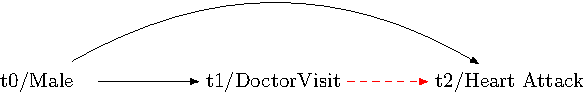
\includegraphics[width=0.8\textwidth,height=\textheight]{use-rev-causal-diagrams_files/figure-pdf/fig-dag-1-1.pdf}

}

\caption{\label{fig-dag-1}Causal diagram adapted from Vanderweele et
al.'s three-wave panel design (VanderWeele et al.~2020). The dotted red
lines indicates a reduction in bias arising from including baseline
measures for the exposure and outcome. For an unmeasured confounder U to
bias the exposure-outcome association, it would need to do so
independently of these outcome and exposure baseline measures. The graph
clarifies that by measuring confounders before the exposure and the
exposure before the outcome, we reduce the potential for reverse
causation, collider stratification, and mediator biases.}

\end{figure}

\subsubsection{Step 4. Identify Observable Common Causes of the Exposure
and the
Outcome}\label{step-4.-identify-observable-common-causes-of-the-exposure-and-the-outcome}

Next, we must identify and record at wave 0 (baseline) all potential
confounders that could influence both the exposure (e.g., frequency of
attending religious services) and the outcome (e.g., charitable giving).
Proper identification and adjustment for these confounders are crucial
for accurate causal inference.

\begin{enumerate}
\def\labelenumi{\arabic{enumi}.}
\item
  \textbf{Defining Confounders}: Confounders are variables that are
  associated with either the exposure or the outcome, or that might be a
  descendent of a common cause of both. We should exclude from this set
  any variable that is an instrumental variable. For example, in the
  context of religious service attendance and charitable giving,
  socioeconomic status (SES) could be a confounder. Individuals with
  higher SES might be more likely to attend religious services regularly
  and also have greater financial capacity for charitable giving. We
  should ensure that good measures of SES are obtained at baseline.
\item
  \textbf{Measurement of Confounders}: Confounders should be measured at
  baseline (wave 0) to ensure that their relationship with both the
  exposure and outcome is properly understood and accounted for. This
  measurement helps in disentangling the true effect of the exposure on
  the outcome from the effects of these confounding variables.
\item
  \textbf{Grouping Confounders for Efficiency}: To maintain clarity in
  analysis, it is advisable to group confounders under standard labels
  when they have similar functional roles in the causal diagram. For
  instance, demographic factors like age, gender, and education level
  can be grouped together if they serve similar roles in influencing
  both religious service attendance and charitable giving.
\item
  \textbf{Use Causal Diagrams}: Causal diagrams allow us to visualise
  causal relationships among variables.
\item
  \textbf{Minimize Mediation Bias}: Recording confounders before the
  exposure occurs is critical for minimizing mediation bias. Mediation
  bias can arise when a variable is both a confounder and a mediator in
  the causal pathway. By identifying and adjusting for these variables
  at baseline, we can reduce the risk of incorrectly attributing the
  effect of the exposure to a mediator.
\end{enumerate}

\subsubsection{Step 5. Gather data for proxy variables of unmeasured
common causes at the baseline
wave}\label{step-5.-gather-data-for-proxy-variables-of-unmeasured-common-causes-at-the-baseline-wave}

If any unmeasured confounders influence both the exposure and outcome,
but we lack direct measurements, we should make efforts to include
proxies for them. Even if this strategy cannot eliminate all bias from
unmeasured confounding, it will generally reduce bias.

\subsubsection{Step 6. State the target population for whom the causal
question
applies}\label{step-6.-state-the-target-population-for-whom-the-causal-question-applies}

We need to define for whom our causal inference applies. For this
purpose, it is helpful to distinguish the concepts of source population
and target population and between the concepts of generalisability and
transportability.

\begin{enumerate}
\def\labelenumi{\arabic{enumi}.}
\item
  \textbf{The source population} is the population from whom our sample
  is drawn.
\item
  \textbf{The target population} is the larger population for whom we
  aim to apply our study's results. The closer the source population
  matches the target population in structural features relevant to our
  causal questions, the stronger our causal inferences about the target
  population will be.
\item
  \textbf{Generalisability}: when the causal effect estimated from a
  sample applies to the target population beyond the sample population,
  we say the causal effect estimates are generalisable. This concept is
  also known as ``external validity.''
\end{enumerate}

Let \(PATE\) denote the population average treatment effect for the
target population. Let \(ATE_{\text{source}}\) denote the average
treatment effect in the source population. Let \(W\) denote a set of
variables upon which the source and target population structurally
differ. We say that results \emph{generalise} if there is a function
such that:

\[PATE =  f(ATE_{\text{source}}, W)\]

\begin{enumerate}
\def\labelenumi{\arabic{enumi}.}
\setcounter{enumi}{3}
\tightlist
\item
  \textbf{Transportability}: when causal effects estimates may
  generalise to different settings and populations from which the source
  population was sampled, we say effects are transportable. Where \(T\)
  denotes a set of variables upon which the source and the target
  population structurally differ, we say that results are transportable
  if there is a function such that
\end{enumerate}

\[ATE_{\text{target}} \approx f(ATE_{\text{source}}, T)\]

This function similarly maps the average treatment effect from the
source population to a target population. The function over \(T\) might
be more complex, as it must handle potential heterogeneity of effects
and unobserved sources of bias. To assess transportability, we generally
require information about the source and target populations and a
specialist understanding.

\subsubsection{Step 7. Retain Sample}\label{step-7.-retain-sample}

Maintaining a stable sample over the course of a three-wave panel study
is critical for ensuring the validity of causal inferences. Panel
attrition, where participants drop out of the study over time, can
introduce significant biases. Therefore, strategies for sample retention
are essential for data collection that is purpose built for causal
inference.

\begin{enumerate}
\def\labelenumi{\arabic{enumi}.}
\item
  \textbf{Developing Tracking Protocols}: Establish robust systems for
  tracking participants over the study period. This involves keeping
  updated records of contact information such as addresses, emails,
  phone numbers, and names, and accounting for changes over time.
  Advanced tracking methods might include periodic contact or follow-ups
  to keep the records current.
\item
  \textbf{Motivational Strategies for Retention}: Implement strategies
  to encourage ongoing participation. This can involve regular
  communication about the study's progress and impact, providing
  incentives for continued participation, or making the process as
  convenient as possible for participants. The key is to engage the
  participants in a way that motivates them to stay involved.
\item
  \textbf{Inclusivity in Participant Engagement}: Ensure that retention
  strategies are inclusive and cater to the diverse needs of the
  population under study. This might involve tailoring communication or
  incentives to different subgroups within the population or addressing
  specific barriers to continued participation that certain groups might
  face.
\item
  \textbf{Use Local Knowledge}: Engage with specialists who have
  in-depth knowledge of the population under study. They can provide
  insights into the most effective strategies for retaining different
  groups within the population.
\item
  \textbf{Participant Feedback and Adaptation}: Incorporate feedback
  from participants to improve retention strategies. This could involve
  regular surveys or feedback sessions to understand participants'
  experiences and adjust the study procedures accordingly.
\item
  \textbf{Addressing Potential Bias from Attrition}: Even with robust
  retention strategies, some degree of attrition is often inevitable.
  Plan for potential attrition from the outset by over-sampling and
  always include methods for adjusting for it at the analysis phase.
\item
  \textbf{Continual Monitoring and Response}: Continuously monitor the
  rate and patterns of attrition throughout the study and implement
  responsive strategies as needed. This could involve targeted
  re-engagement efforts or adjustments in study procedures to address
  emerging challenges.
\item
  \textbf{Documentation and Reporting}: Carefully document all retention
  efforts and the patterns of attrition that occur in the study. This
  documentation is crucial for interpreting the study results and for
  informing future research.
\end{enumerate}

Sample retention is mission-critical for preventing bias arising to
panel attrition in three-wave panel designs. Researchers must be aware
of it, and combat it.

\subsection{References}\label{references-1}



\end{document}
